\chapter{Análisis colección \#BLM}
\label{chap:blm}

\lettrine{E}{s} importante no olvidar el objetivo inicial de todo el trabajo previo de los anteriores capítulos. Aunque el desarrollo de la herramienta de perfilado es un fin en sí mismo, y se puede aplicar a más casos de uso que el tratamos nosotros, nuestra verdadera motivación consiste en aplicar esta herramienta de perfilado automático de usuarios para obtener información y poder razonar sobre el movimiento social \acrshort{blm}.

Concretamente, en este capítulo se aplicará nuestro sistema para conocer mejor el tipo de usuarios que publicaban en el corpus, en idioma español, construido por \citet{heritage_BLM} en 2020 a modo de archivo social sobre sobre las discusiones acerca de los conflictos raciales motivados por el asesinato de George Floyd. Este corpus se encuentra disponible en \url{https://www.dc.fi.udc.es/~david/hdh2021/}.

\subsection{Procesado corpus}

Al descargar el corpus de la dirección anterior, este viene distribuido entre múltiples archivos XML por cada \textit{thread} o <<hilo>> del subreddit de BLM. Esta agrupación tiene sentido ya que cada <<hilo>> representa un tópico distinto y los comentarios en cada uno tienen un contexto común. Sin embargo, para nuestra finalidad de perfilar cada usuario de la colección tiene mayor importancia usar el mayor número de publicaciones por usuario para que de esta forma las predicciones tengan mayor fiabilidad.
% \begin{verbatim}
% <thread>
%     <id>477</id>
%     <relevant-posts>
%         <id>479</id>
%     </relevant-posts>
%     <posts>
%         <post>
%             <id>479</id>
%             <author>478</author>
%             <body>
%                 >Eso no se de donde lo sacás. Si quieren prohibir el racismo ...
%             </body>
%         </post>
%         ...
%     </posts>
% </thread>

% \end{verbatim}

En este sentido, se procedió a crear un único archivo CSV, con dos columnas: identificador del usuario y texto de la publicación. Este CSV contendrá todas las publicaciones de cada autor de la colección sin tener en cuenta el hilo concreto de cada una. Es importante señalar que no se agrupan las publicaciones de cada autor en una fila, sino que cada publicación de partida se escribe en una fila distinta del CSV. De esta forma, al tener las publicaciones de cada autor separadas, cada algoritmo de perfilado se encarga de unirlas y preprocesarlas de la manera oportuna.

\section{Aplicación}
Posteriormente, tras haber creado este archivo CSV con el conjunto de todas las publicaciones de los autores de \acrshort{blm} ya se puede subir a la aplicación para perfilar el corpus. Para ello, arrancamos la aplicación en el entorno local y accedemos desde un navegador a la dirección de \textit{localhost} en el puerto 3000. Tras este paso se podrá ver una página de inicio como la de la figura \ref{fig:app/home}. En cada figura de esta sección se mostrarán dos subfiguras con las vistas de la aplicación desde: ordenador de sobremesa (\textit{desktop}) y móvil (\textit{mobile}).

\begin{figure}[H]
  \centering
  \begin{subfigure}{0.7\textwidth}
       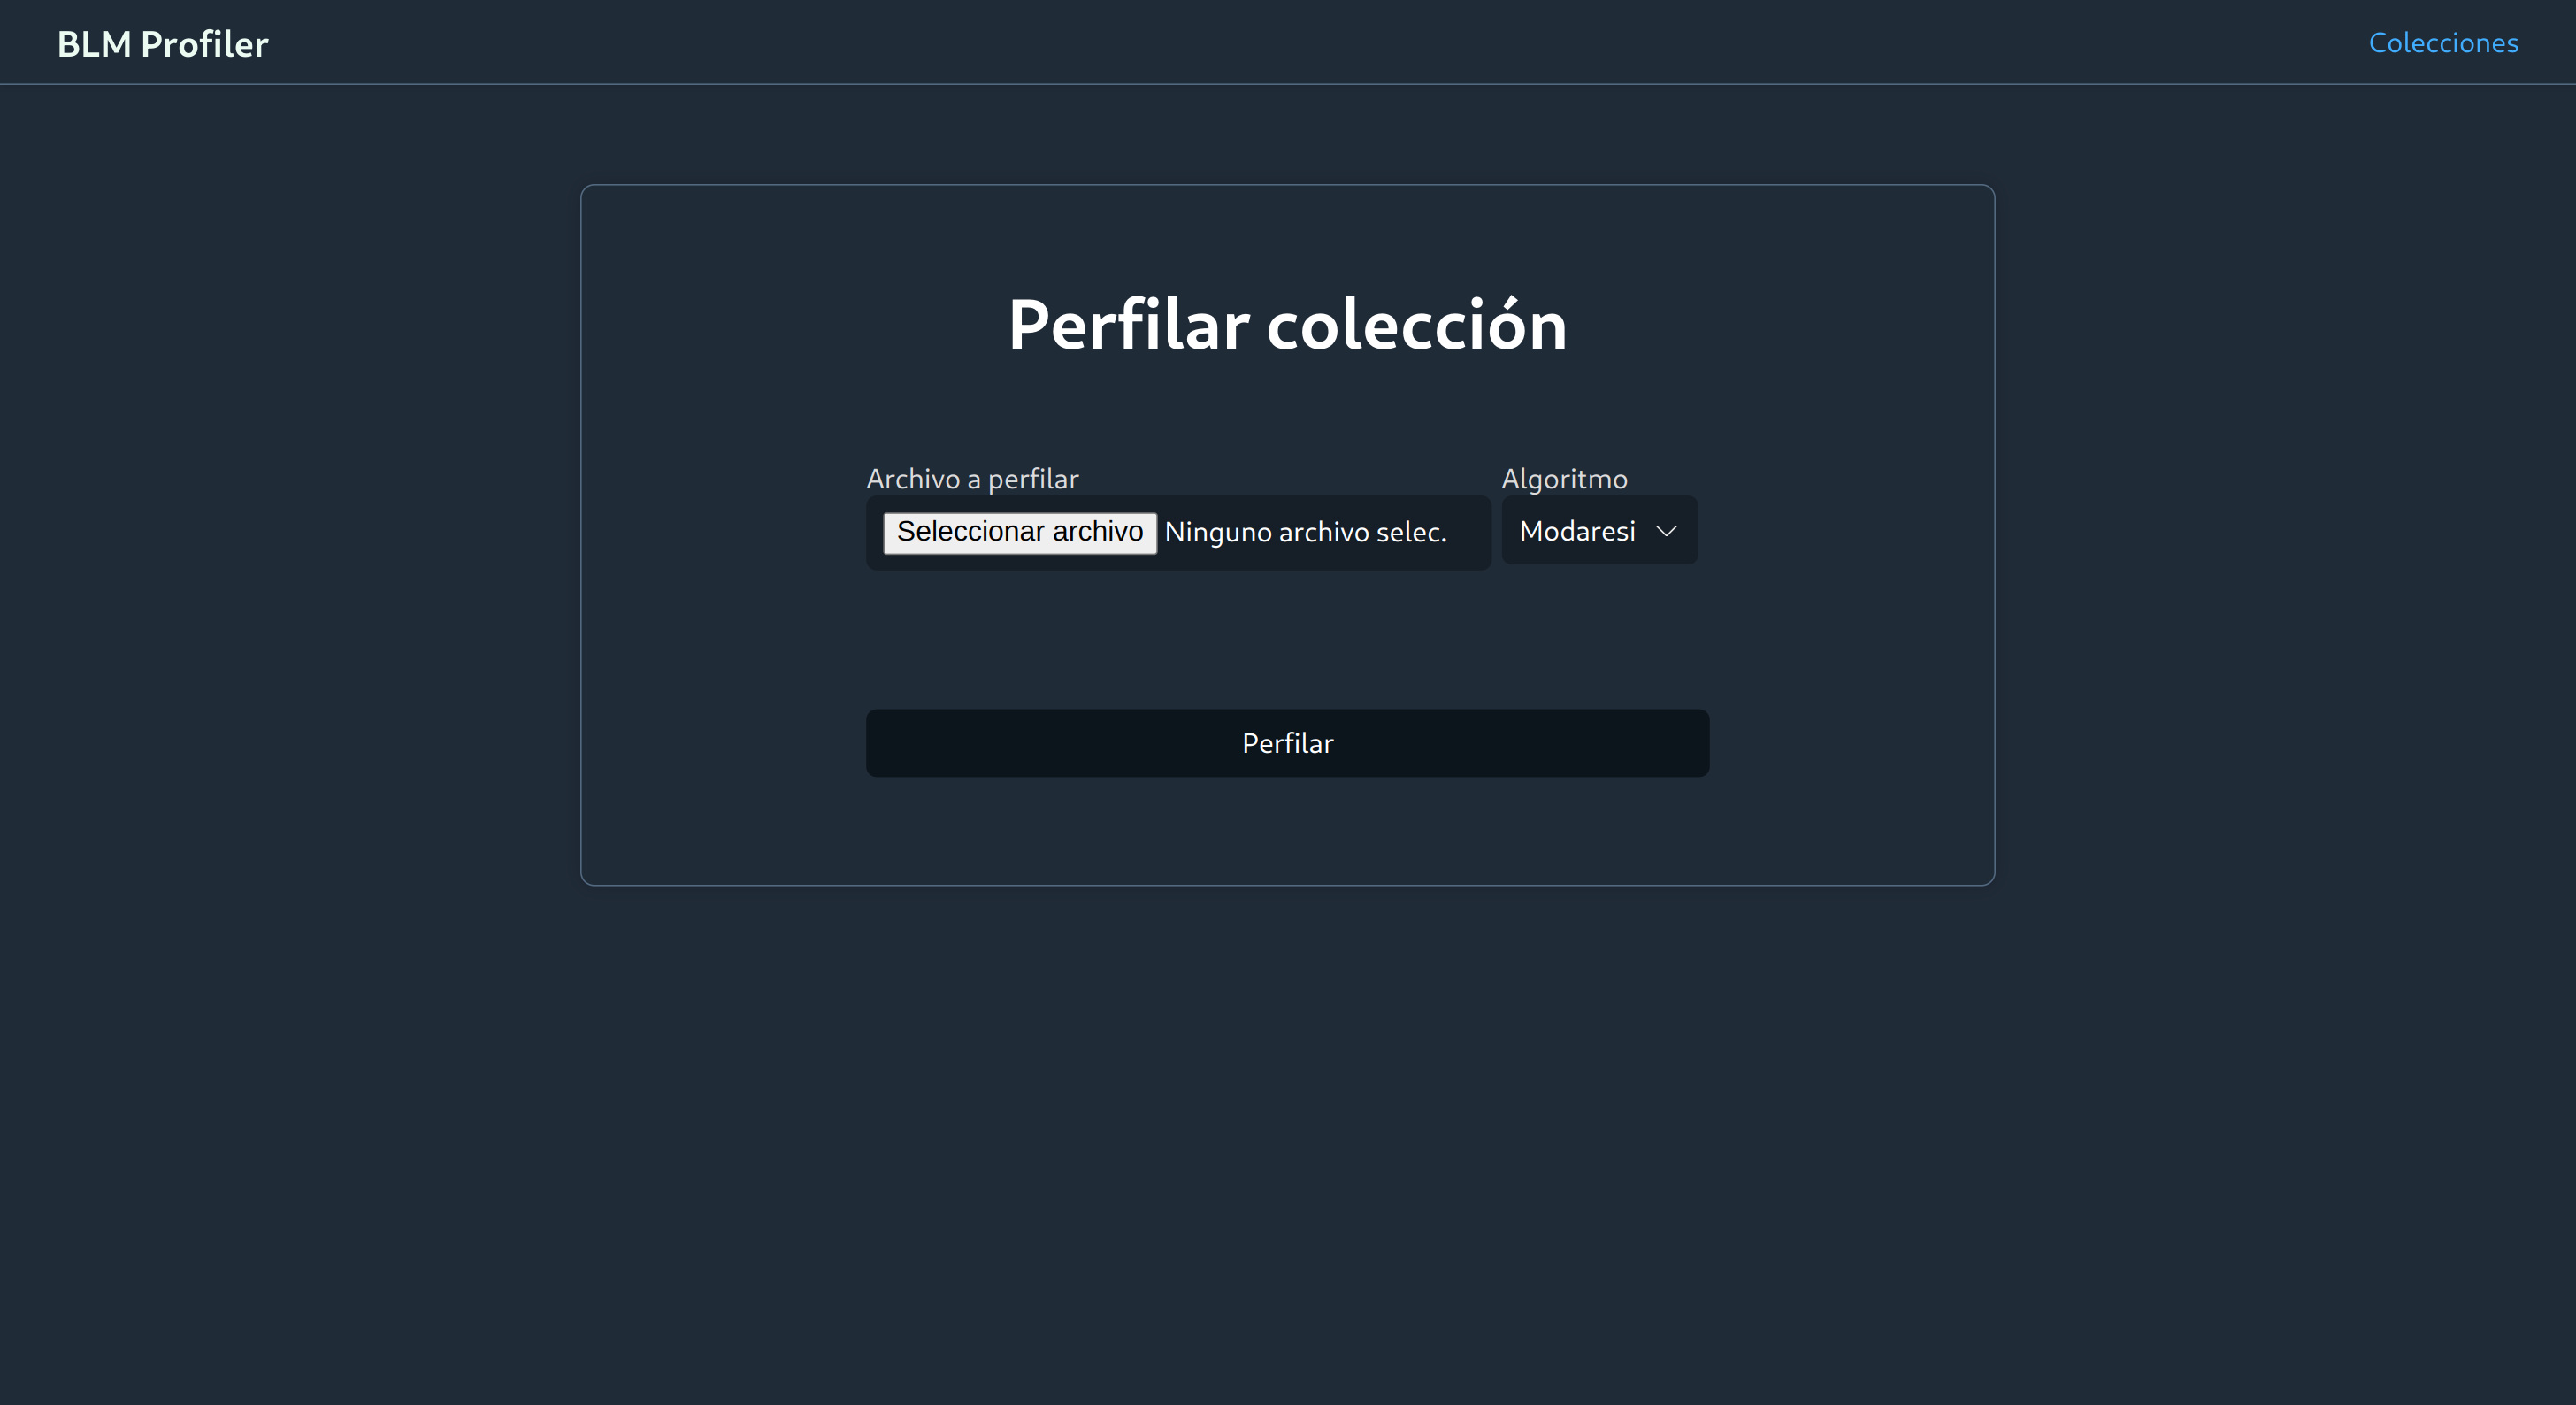
\includegraphics[width=\textwidth]{imaxes/capturas-app/desktop/home.png}
      \caption{\textit{Desktop}} 
  \end{subfigure}
  \begin{subfigure}{0.2215\textwidth}
       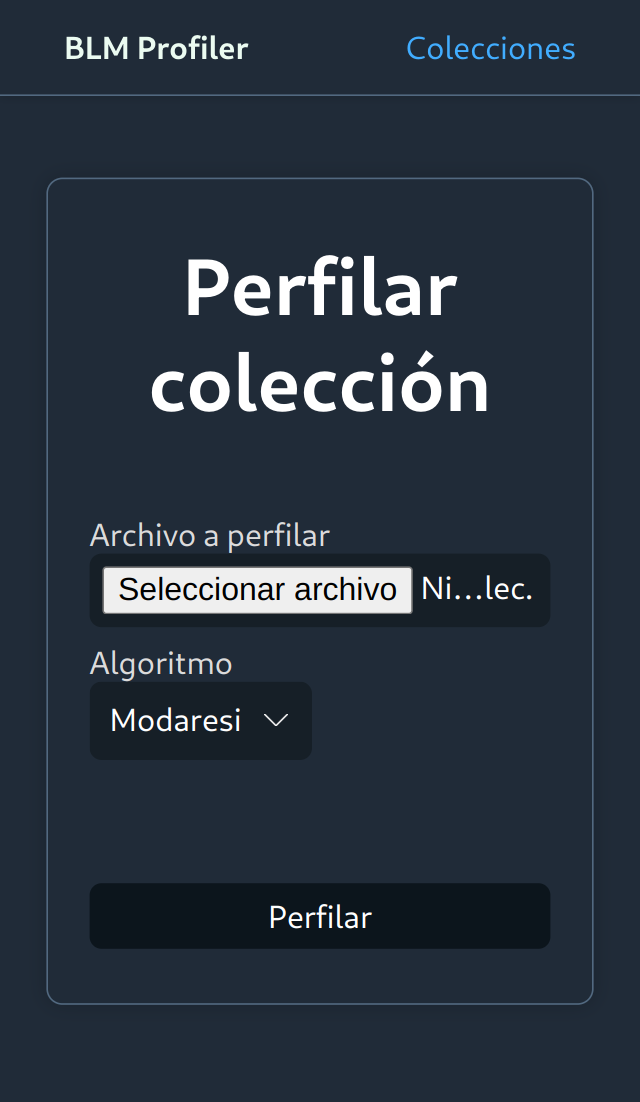
\includegraphics[width=\textwidth]{imaxes/capturas-app/mobile/home.png}
      \caption{\textit{Mobile}} 
  \end{subfigure}
  \caption{Página de inicio.}
  \label{fig:app/home}
\end{figure}
\subsection{Perfilado del corpus}

En esta página se puede ver un formulario con dos campos: uno obligatorio que es el selector del fichero que contiene el corpus a perfilar y otro opcional selector para escoger el algoritmo de perfilado deseado, que por defecto será el de <<modaresi>>. Tras seleccionar el fichero que contiene el corpus a perfilar, que debe tener extensión .csv o .txt, se nos mostrará un mensaje en función de si este es válido o no para el perfilado\footnote{Para que el fichero sea válido debe tener al menos dos columnas llamadas \textit{id} y \textit{posts}, que se refieren al identificador del usuario y su publicación.}. En función de ello nos dejará o no perfilar la colección. Tras este paso, podremos hacer click en el botón de perfilar y la página mostrará un \textit{spinner} a modo de carga mientras se perfila la colección, como se puede ver en la figura \ref{fig:app/home-perfilando}.

\begin{figure}[H]
  \centering
  \begin{subfigure}{0.7\textwidth}
       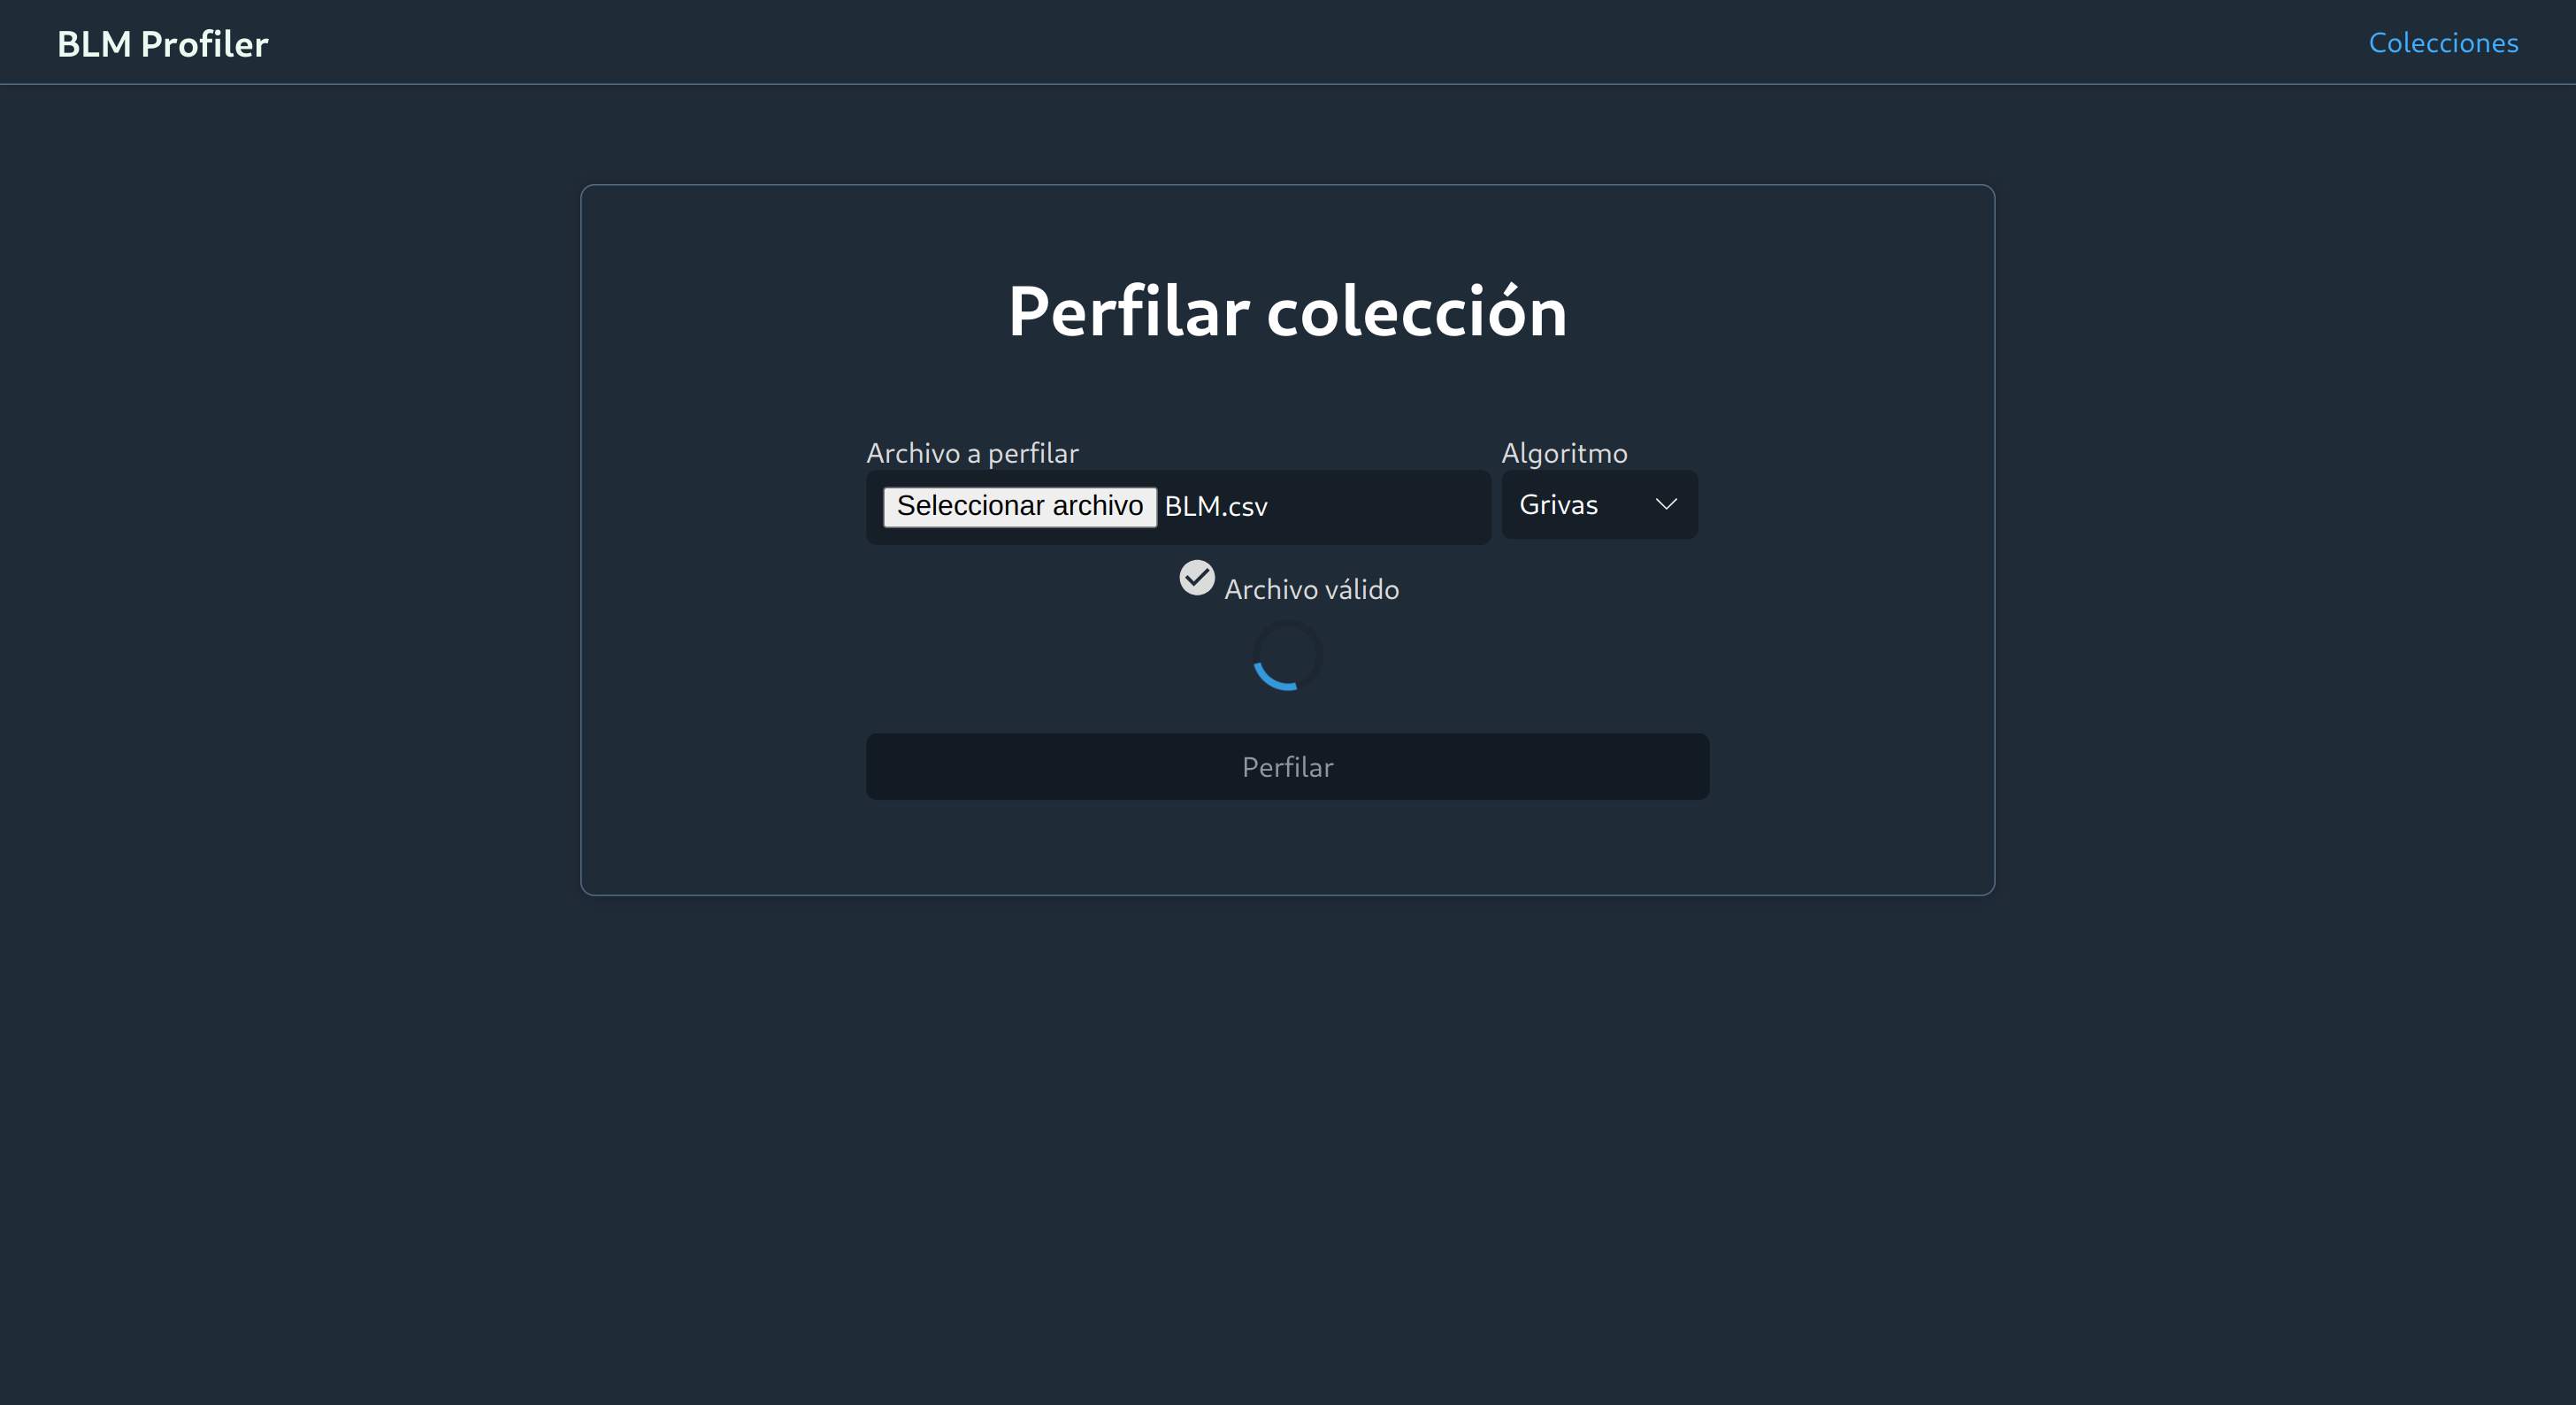
\includegraphics[width=\textwidth]{imaxes/capturas-app/desktop/home_perfilando.png}
      \caption{Desktop} 
  \end{subfigure}
  \begin{subfigure}{0.2215\textwidth}
       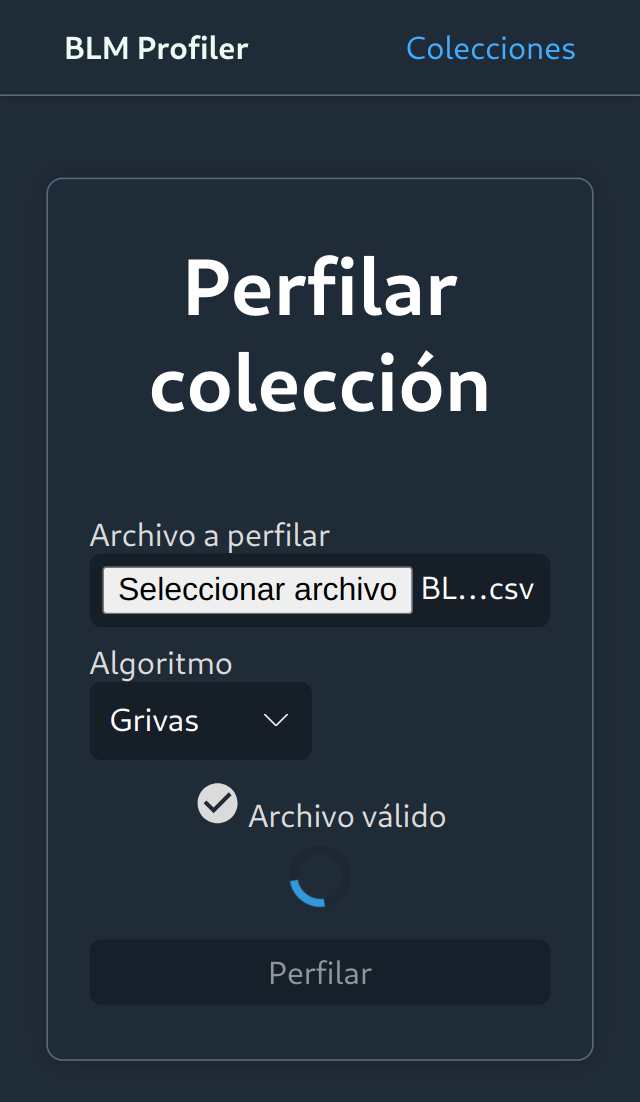
\includegraphics[width=\textwidth]{imaxes/capturas-app/mobile/home_perfilando.png}
      \caption{Mobile} 
  \end{subfigure}
  \caption{Página de inicio mientras se perfila una colección.}
  \label{fig:app/home-perfilando}
\end{figure}
\subsection{Visualización de resultados}

Cuando termine el perfilado la aplicación nos redirigirá al \textit{dashboard} o cuadro de mando de la misma que se puede ver en la figura \ref{fig:app/dashboard}.

\begin{figure}[H]
  \centering
  \begin{subfigure}{0.7\textwidth}
   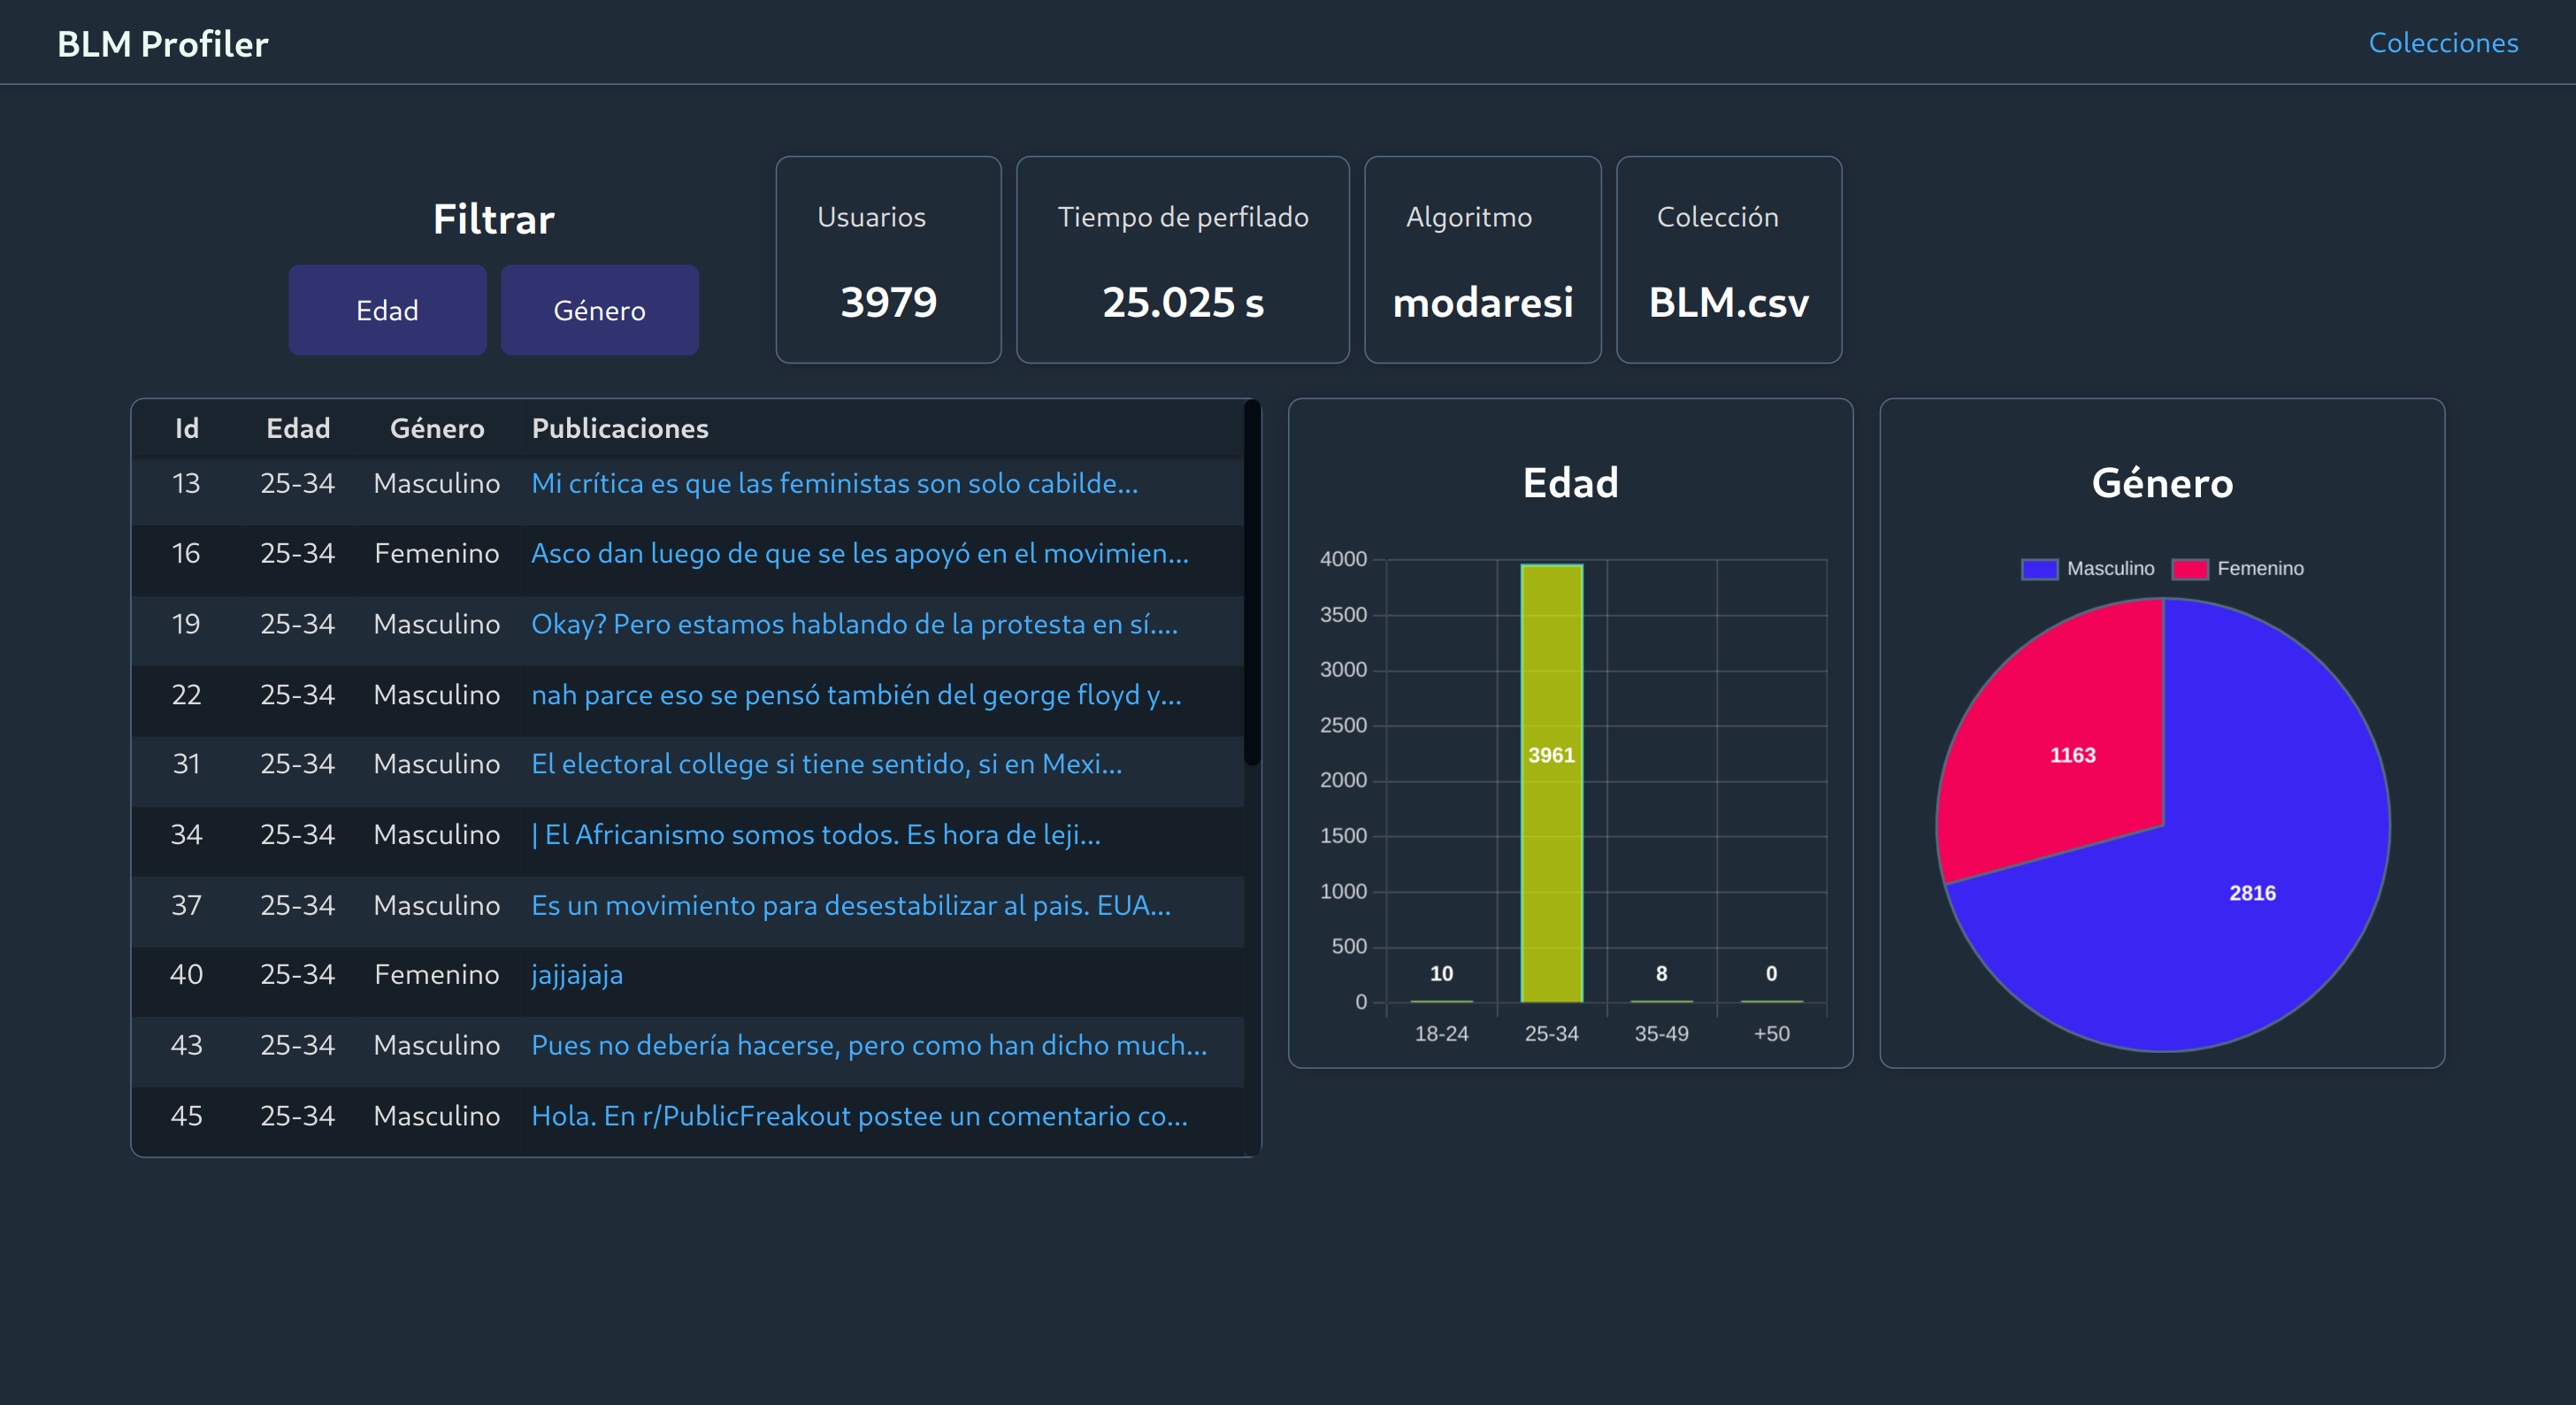
\includegraphics[width=\textwidth]{imaxes/capturas-app/desktop/dashboard.png}
  \caption{\textit{Desktop}} 
  \end{subfigure}
  \begin{subfigure}{0.2215\textwidth}
   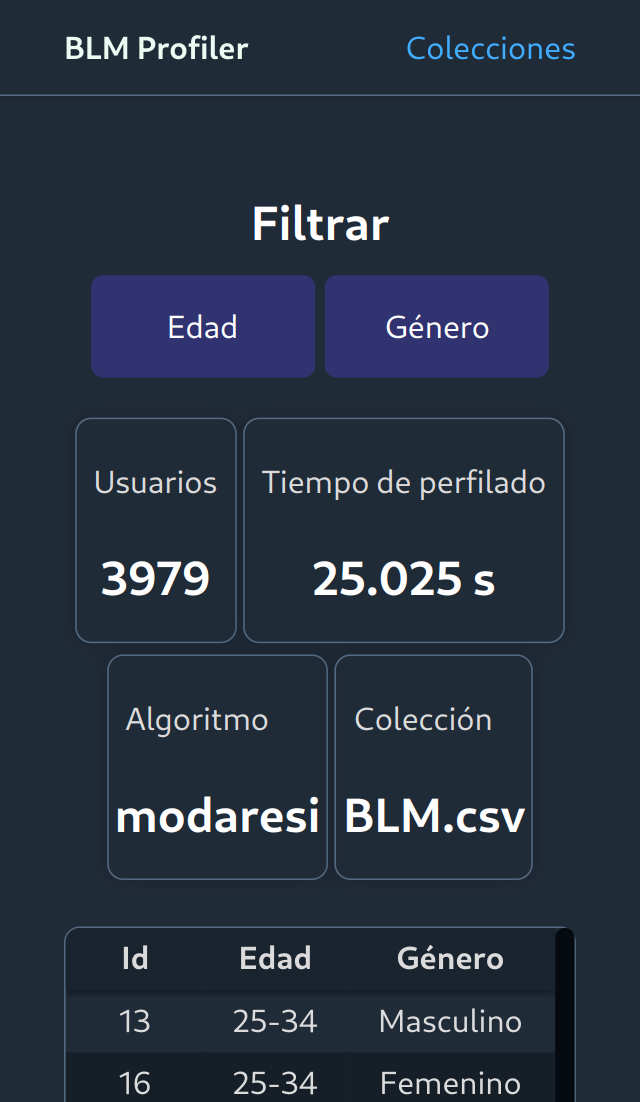
\includegraphics[width=\textwidth]{imaxes/capturas-app/mobile/dashboard.png}
  \caption{\textit{Mobile}} 
  \end{subfigure}
  \caption{\textit{Dashboard} de la colección perfilada.}
  \label{fig:app/dashboard}
\end{figure}

Como podemos ver en la parte de abajo tenemos una tabla y dos gráficos. En el gráfico de barras se puede ver la distribución de los usuarios del corpus según su edad, hay cuatro barras para cuatro rangos de edad distintos. En el gráfico en forma de tarta, en cambio, se muestra la distribución de los usuarios en función del género de los mismos. La tabla, por otra parte, es un listado de todos los usuarios del corpus en el que se muestra el id del mismo\footnote{Correspondiente a la columna id del archivo de subida de la colección}, el género y edad con los que fue clasificado y una muestra de una publicación del usuario en forma de enlace, que explicaremos más adelante.

Luego, en la parte superior, se encuentran varias tarjetas que presentan detalles generales sobre la colección, tales como el tiempo de perfilado, el algoritmo utilizado, el nombre del archivo de subida y el número total de usuarios.

\subsubsection{Filtrado de usuarios por categorías}
Por último, al inicio de la página se encuentra un texto titulado <<Filtrar>> y debajo podemos ver dos botones. Al situar el ratón sobre cualquiera de ellos veremos como realmente son botones desplegables en los que se presentan los posibles filtros para cada categoría. Al seleccionar un filtro de alguna de las categorías veremos como se añade un elemento después de las tarjetas de la colección, que indica el filtro concreto escogido para esa categoría. En la figura \ref{fig:app/dashboard-filtered}, podemos ver el aspecto del filtro añadido.

\begin{figure}[H]
  \centering
  \begin{subfigure}{0.7\textwidth}
   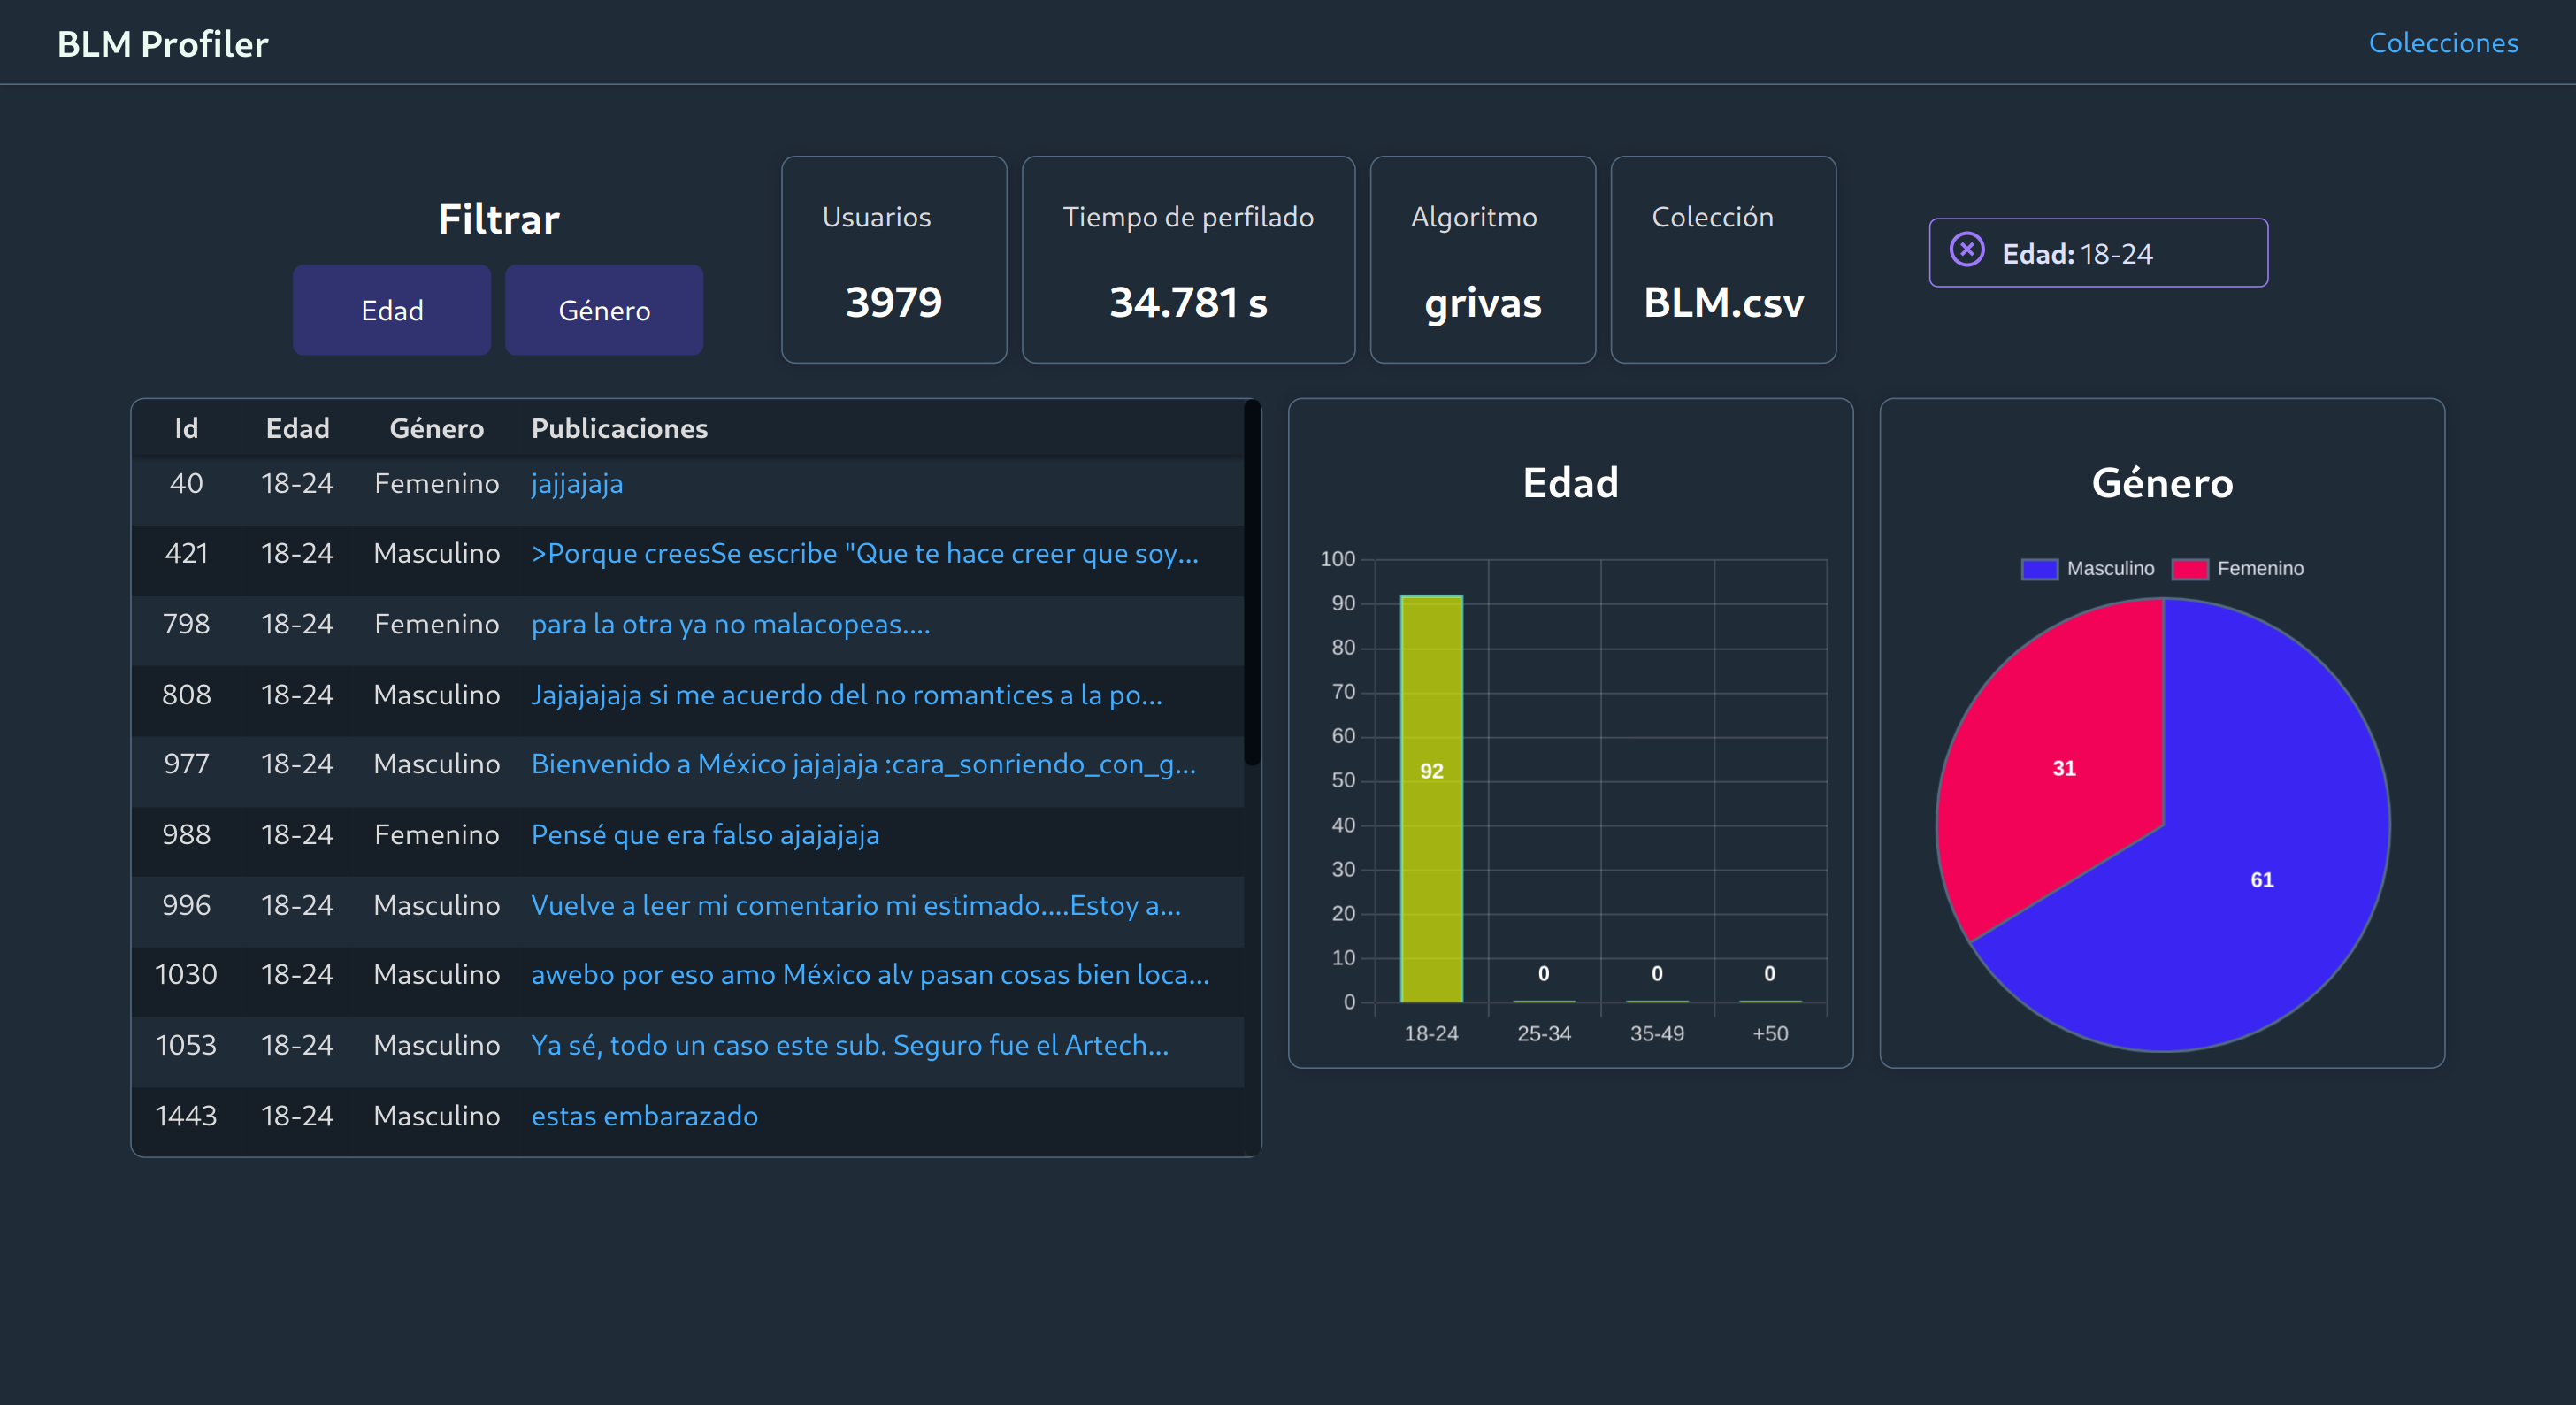
\includegraphics[width=\textwidth]{imaxes/capturas-app/desktop/dashboard-perfilado-edad.png}
  \caption{\textit{Desktop}} 
  \end{subfigure}
  \begin{subfigure}{0.223\textwidth}
   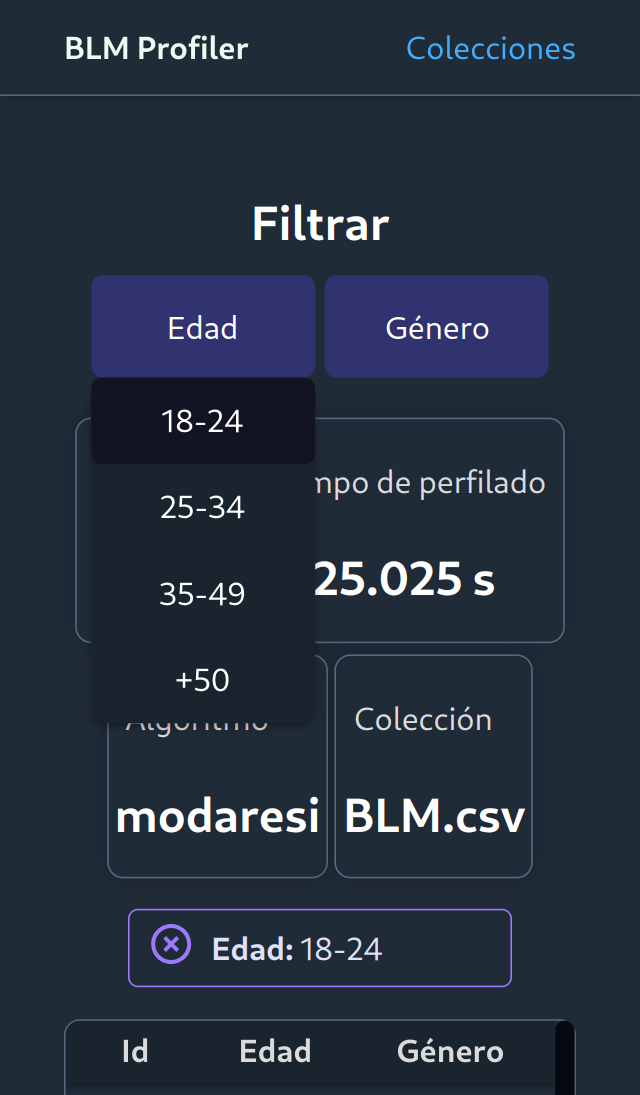
\includegraphics[width=\textwidth]{imaxes/capturas-app/mobile/dashboard-filtrado-edad.png}
  \caption{\textit{Mobile}} 
  \end{subfigure}
  \caption{\textit{Dashboard} de la colección perfilada filtrado únicamente por edad.}
  \label{fig:app/dashboard-filtered}
\end{figure}

Como se puede apreciar en este caso, el proceso de filtrado afecta a la lista de usuarios y a ambos gráficos. Por un lado, en la lista, podemos observar que únicamente se muestran usuarios cuyas edades se sitúan en el rango de 18-24 años. En el gráfico de edad, el filtrado por una grupo de la misma categoría no es especialmente interesante, ya que no nos aporta información nueva. Sin embargo, en el gráfico de género el filtrado por edad nos permite estudiar como cambia la distribución del género de los usuarios en función del rango de edad de los mismos.

Otra opción relevante, es la de filtrar el \textit{dashboard} por ambas categorías. Como ya hemos comentado en los gráficos nos brindaría ninguna información nueva. Por el contrario, al realizar este filtrado podemos estudiar el tipo de publicaciones que realiza un grupo demográfico concreto lo que también nos aporta pistas sobre los criterios que se emplean en el perfilado de cada grupo. En la figura \ref{fig:app/dashboard-filtered-edad-genero}, se puede contemplar el filtrado en función de ambas categorías.

\begin{figure}[H]
  \centering
  \begin{subfigure}{0.7\textwidth}
   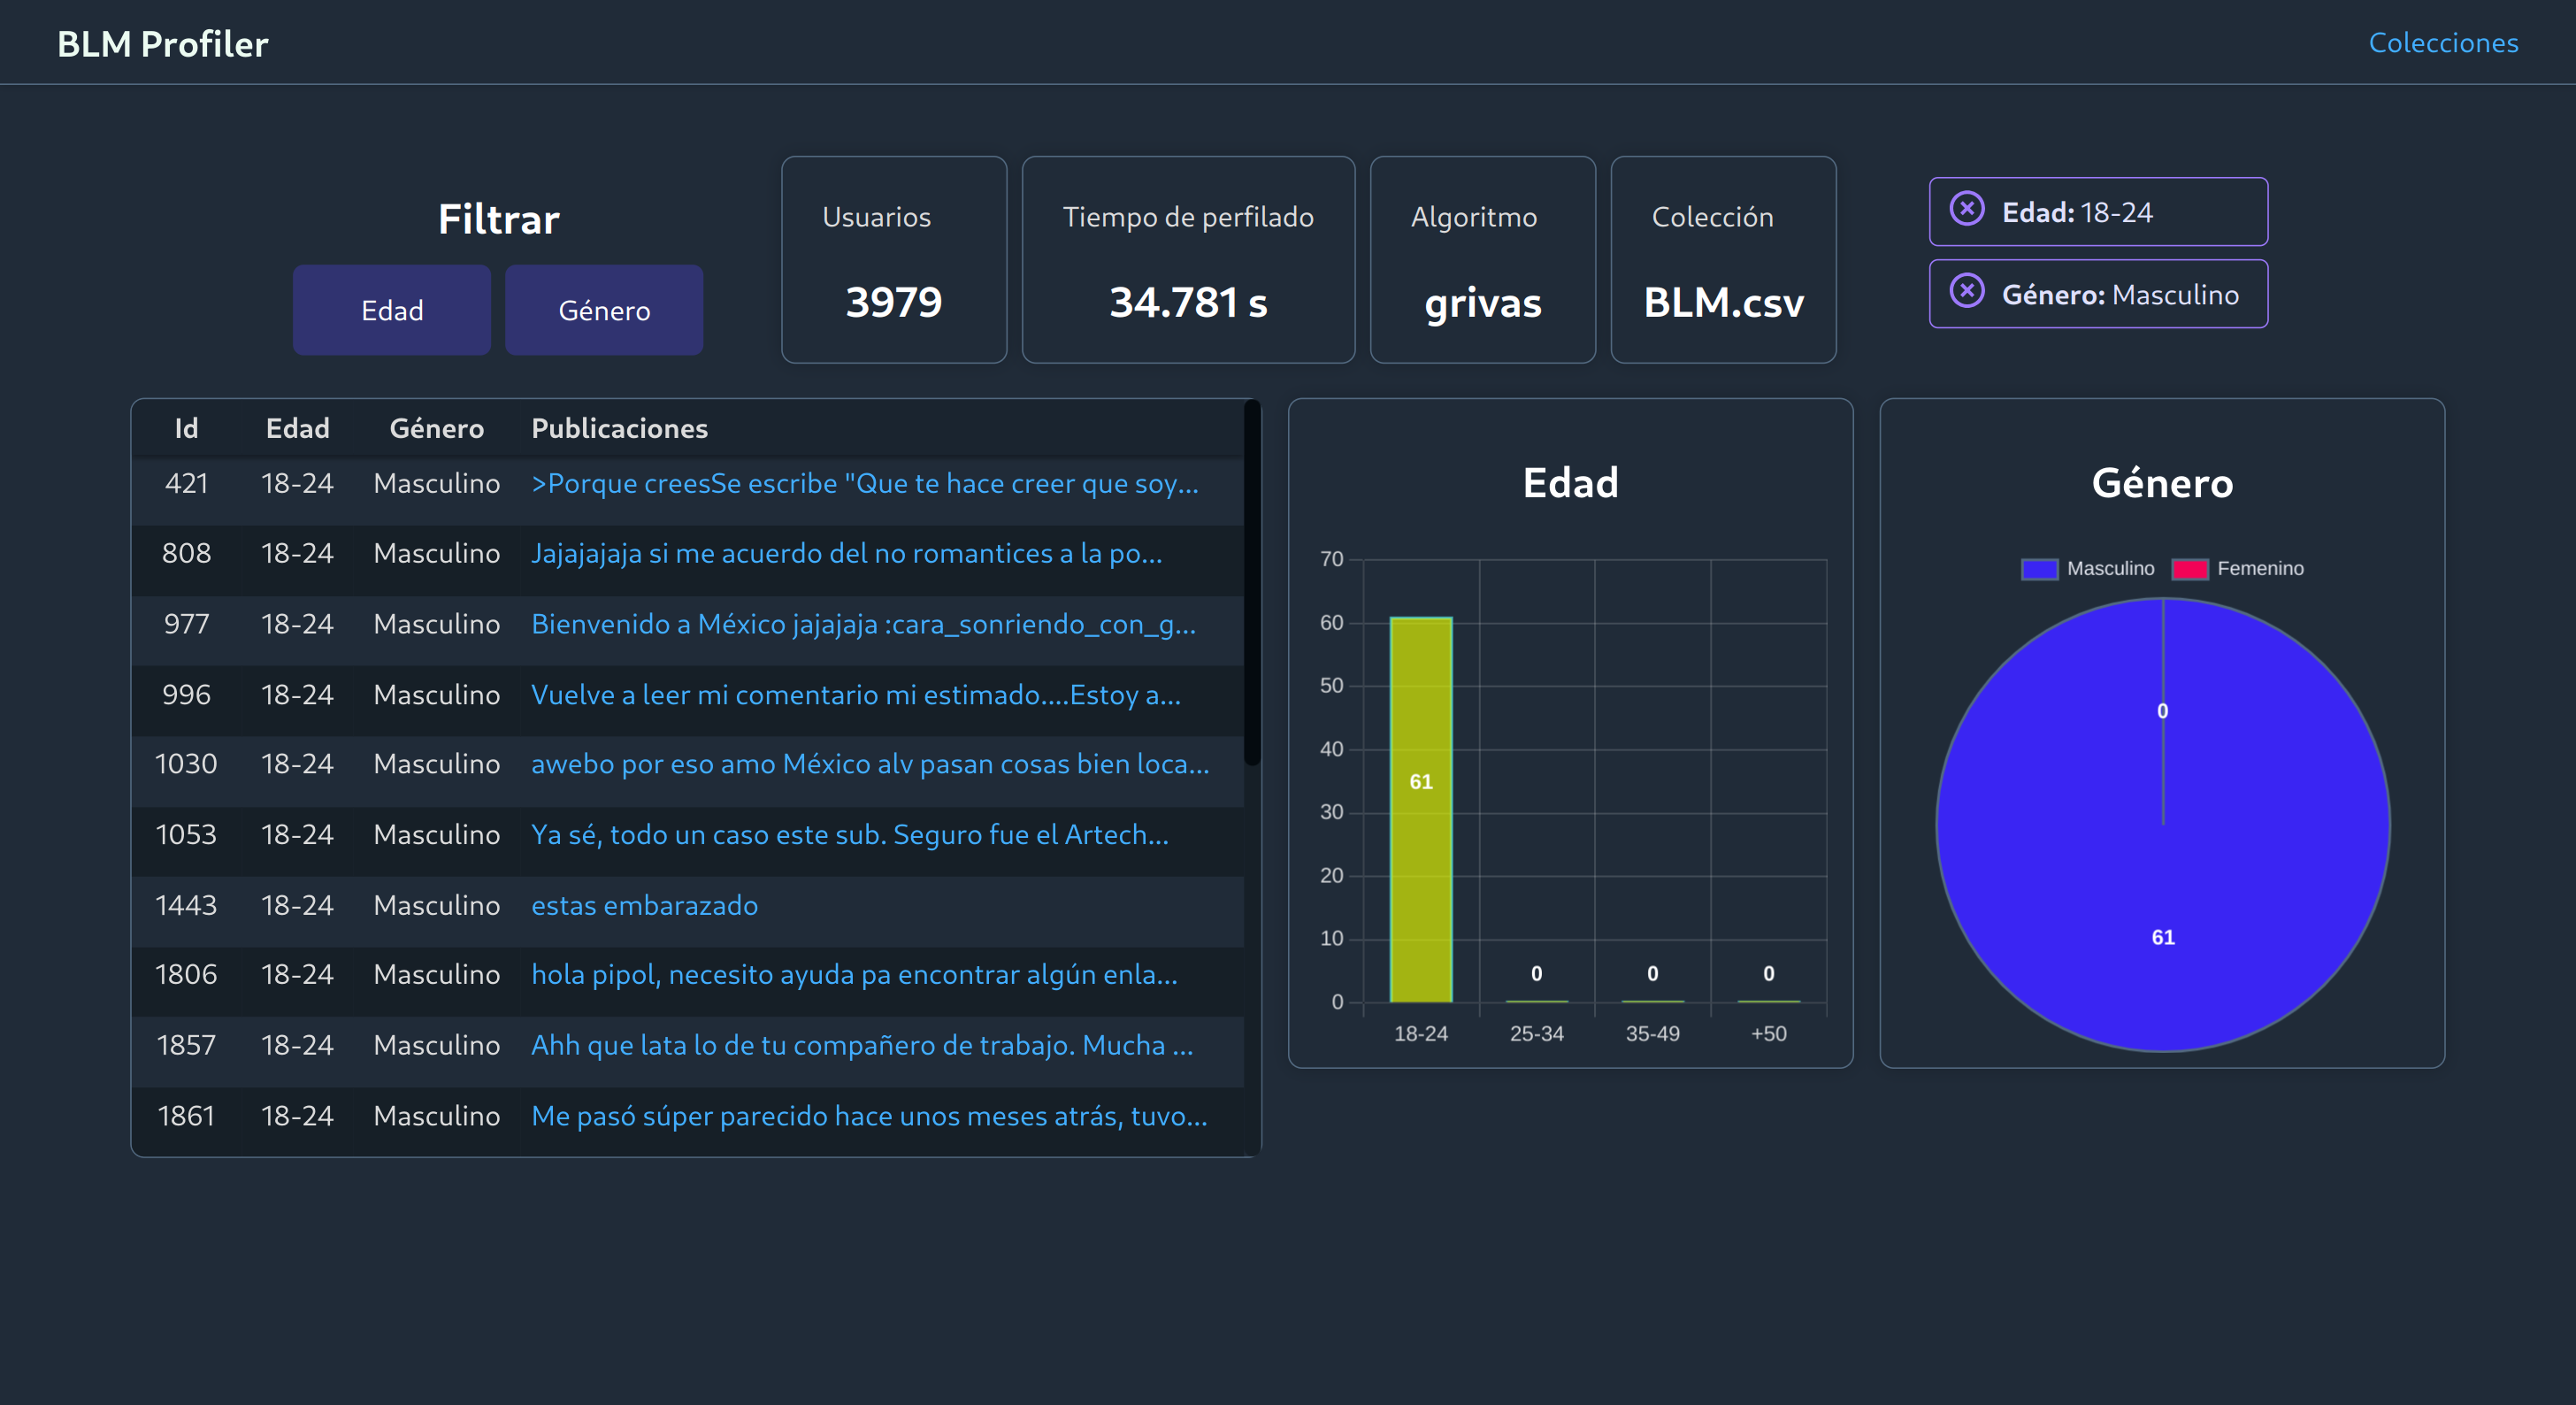
\includegraphics[width=\textwidth]{imaxes/capturas-app/desktop/dashboard-perfilado-edad-genero.png}
  \caption{\textit{Desktop}} 
  \end{subfigure}
  \begin{subfigure}{0.223\textwidth}
   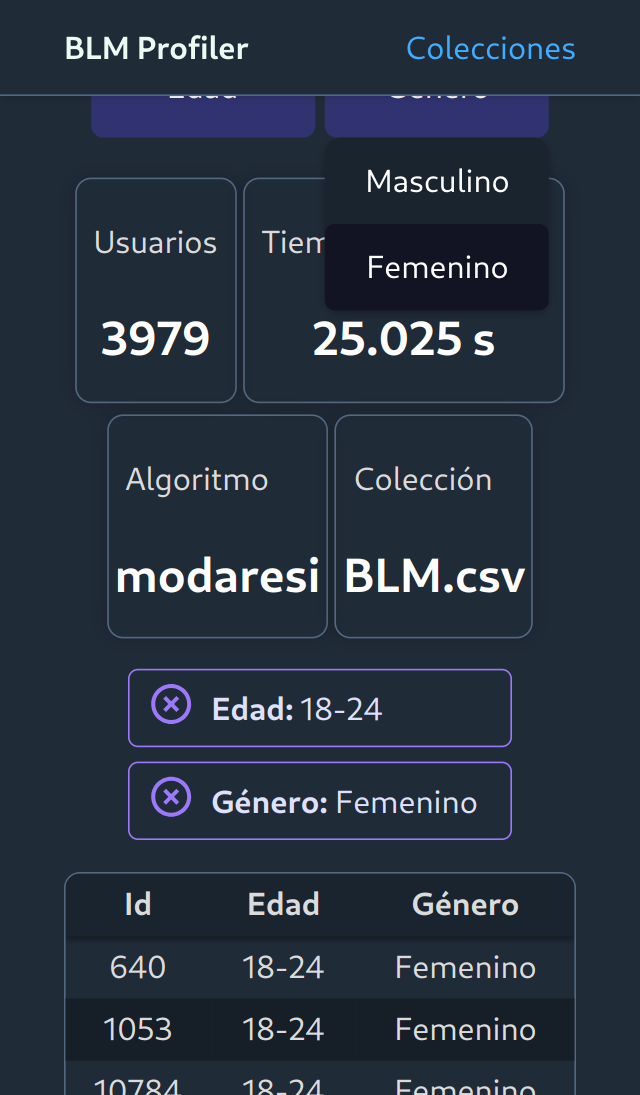
\includegraphics[width=\textwidth]{imaxes/capturas-app/mobile/dashboard-filtrado-edad-genero.png}
  \caption{\textit{Mobile}} 
  \end{subfigure}
  \caption{\textit{Dashboard} de la colección perfilada filtrado por género y edad.}
  \label{fig:app/dashboard-filtered-edad-genero}
\end{figure}

\subsection{Publicaciones de un usuario}
Por ejemplo, si deseáramos examinar el estilo de redacción de un usuario masculino de entre 25 a 34 años, haríamos clic sobre el enlace de la columna <<Publicaciones>> en la versión \textit{desktop}, o directamente seleccionando una fila de la tabla, en la versión \textit{mobile}. Con esta acción podríamos ver las publicaciones del usuario seleccionado en una página similar a la de la figura \ref{fig:app/user-info}.

\begin{figure}[H]
  \centering
  \begin{subfigure}{0.7\textwidth}
   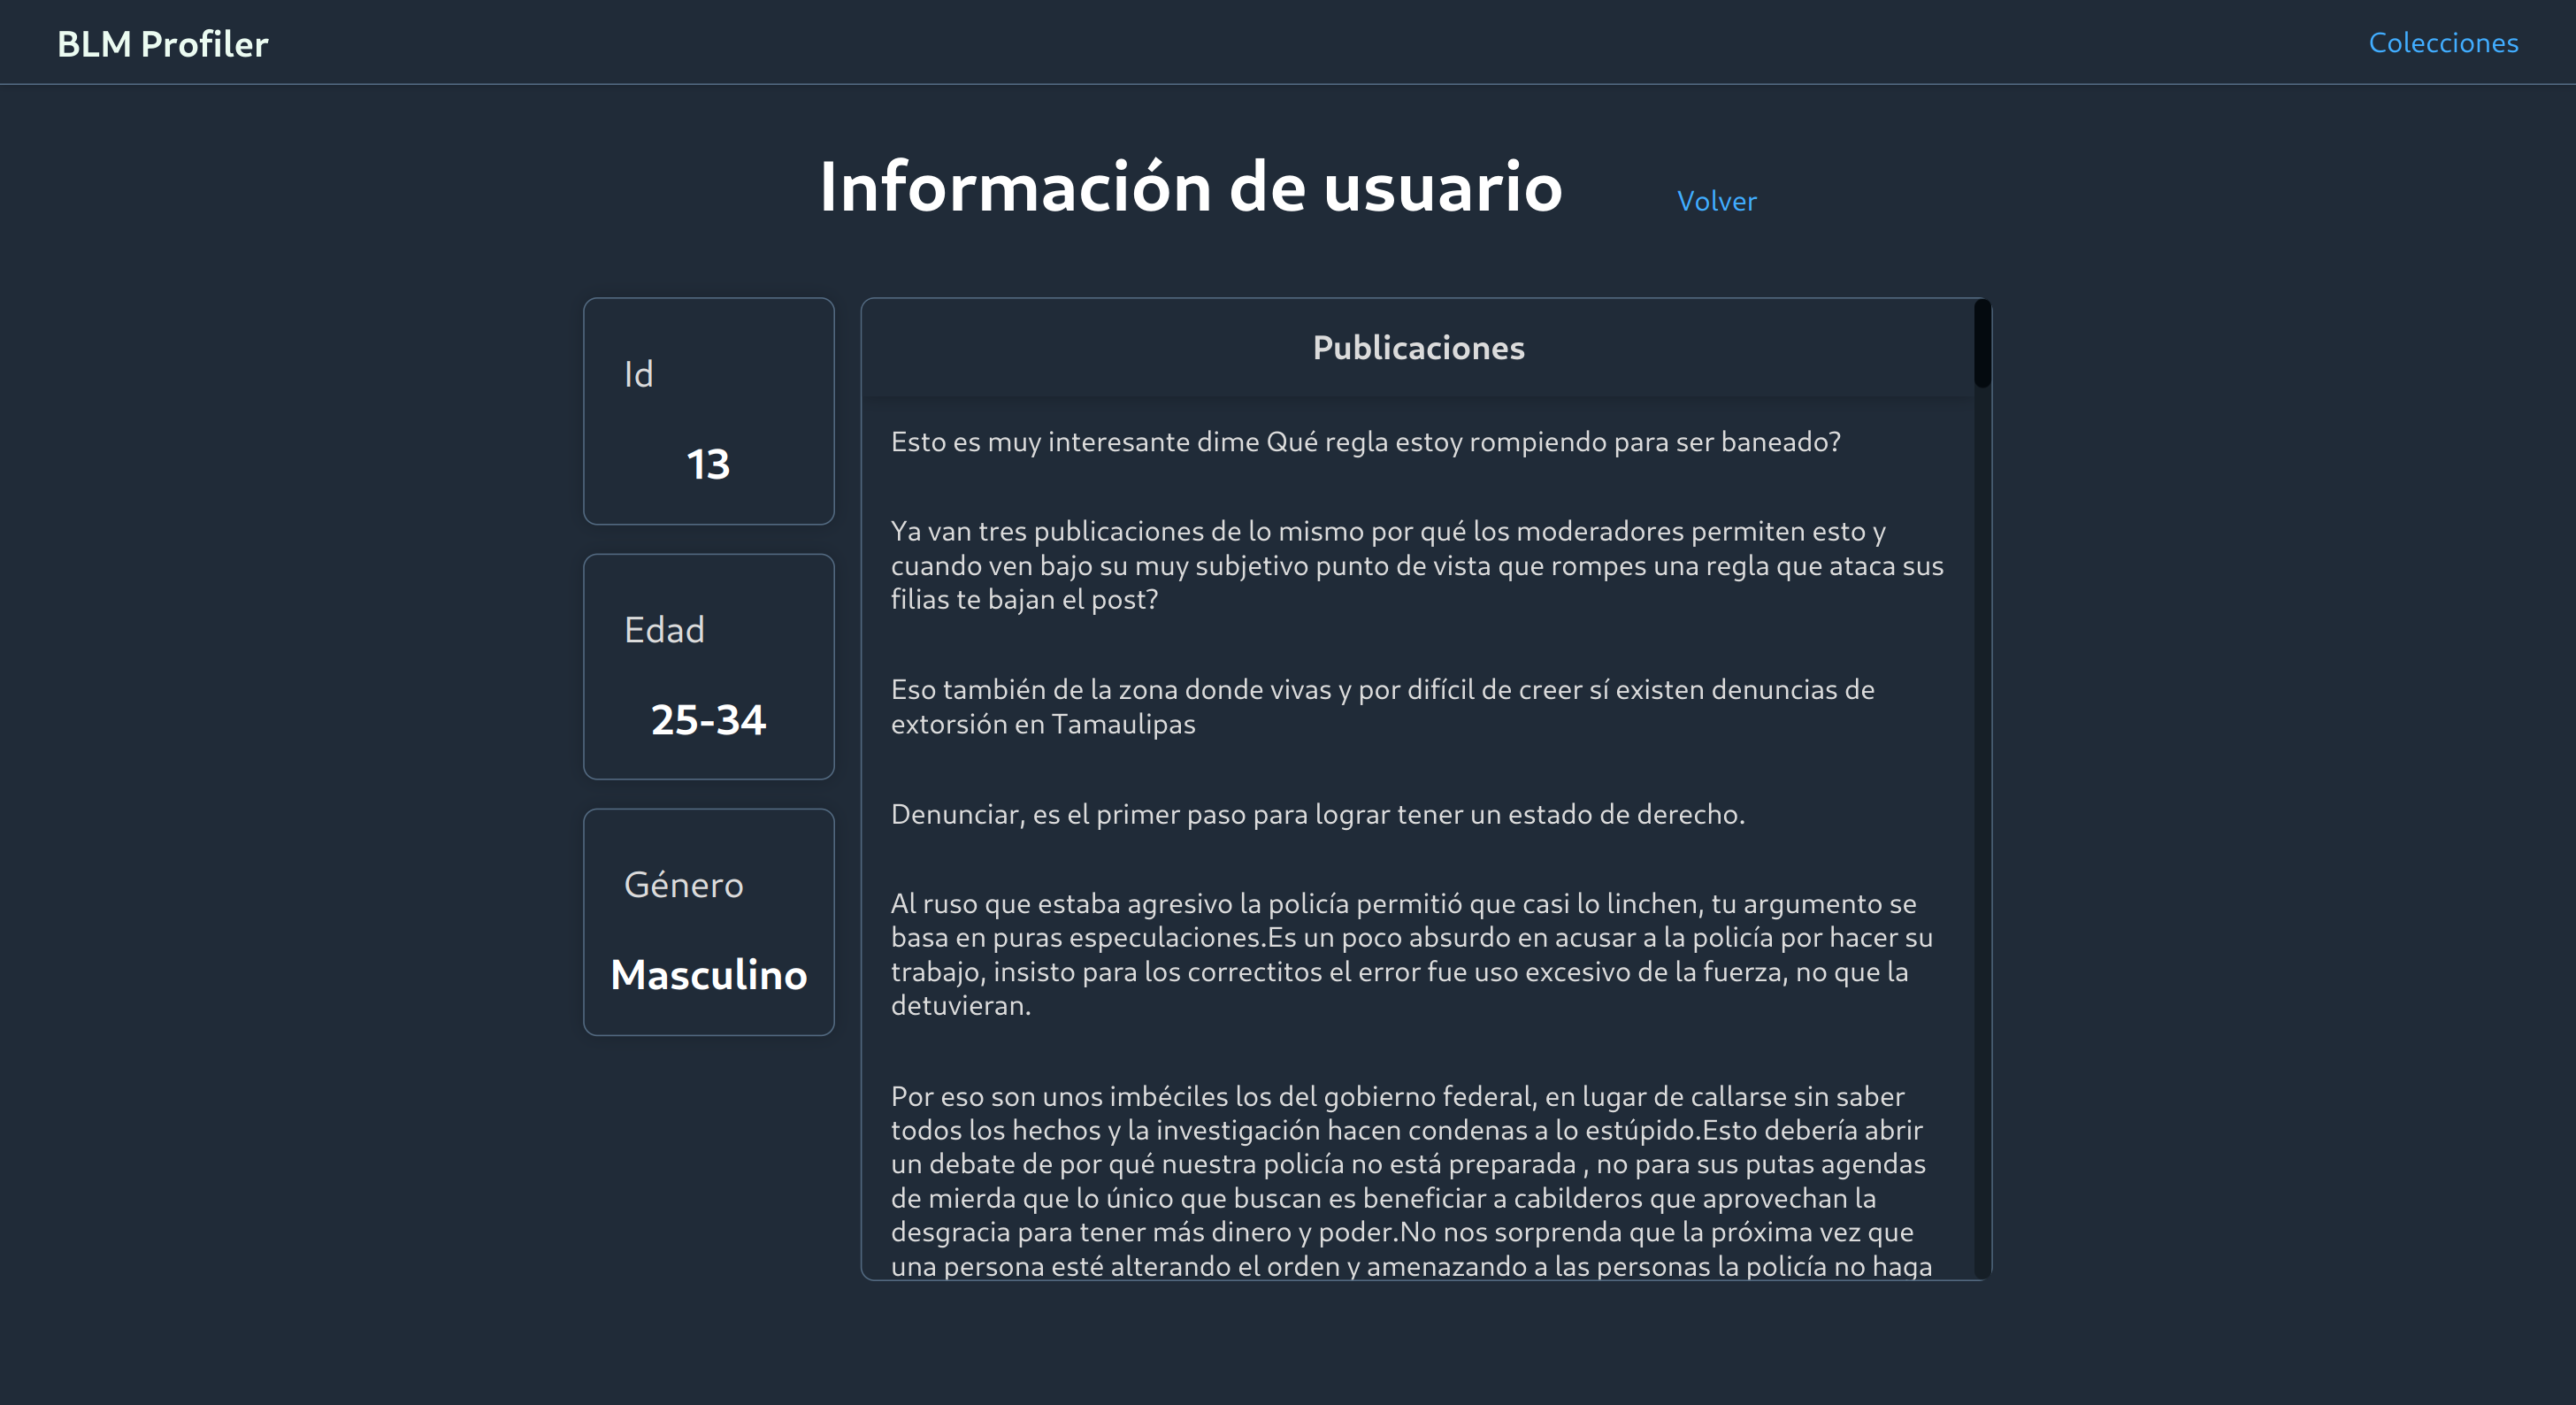
\includegraphics[width=\textwidth]{imaxes/capturas-app/desktop/info-usuario.png}
  \caption{\textit{Desktop}} 
  \end{subfigure}
  \begin{subfigure}{0.223\textwidth}
   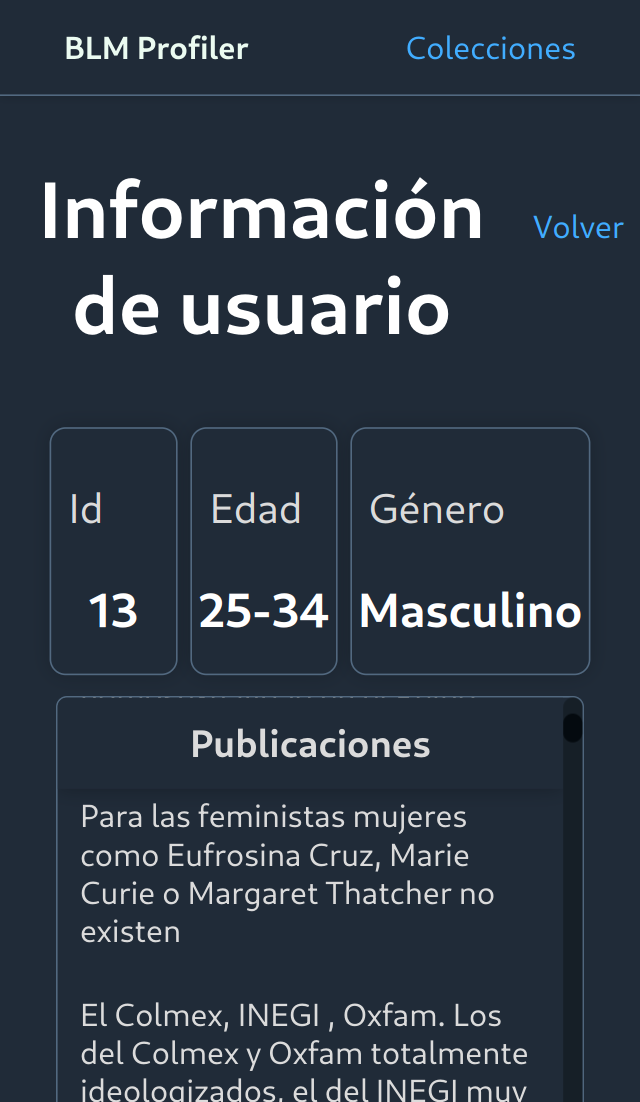
\includegraphics[width=\textwidth]{imaxes/capturas-app/mobile/info-usuario.png}
  \caption{\textit{Mobile}} 
  \end{subfigure}
  \caption{Página de la vista en detalle de un usuario de la colección.}
  \label{fig:app/user-info}
\end{figure}

\subsection{Listado de colecciones}
En cambio, si no deseamos perfilar una colección nueva sino que queremos ver el listado histórico de colecciones ya perfiladas, en la barra de navegación tenemos un enlace, arriba a la derecha, llamado <<Colecciones>> que nos llevará a una página como la de la figura \ref{fig:app/colecciones}. 

\begin{figure}[H]
  \centering
  \begin{subfigure}{0.7\textwidth}
   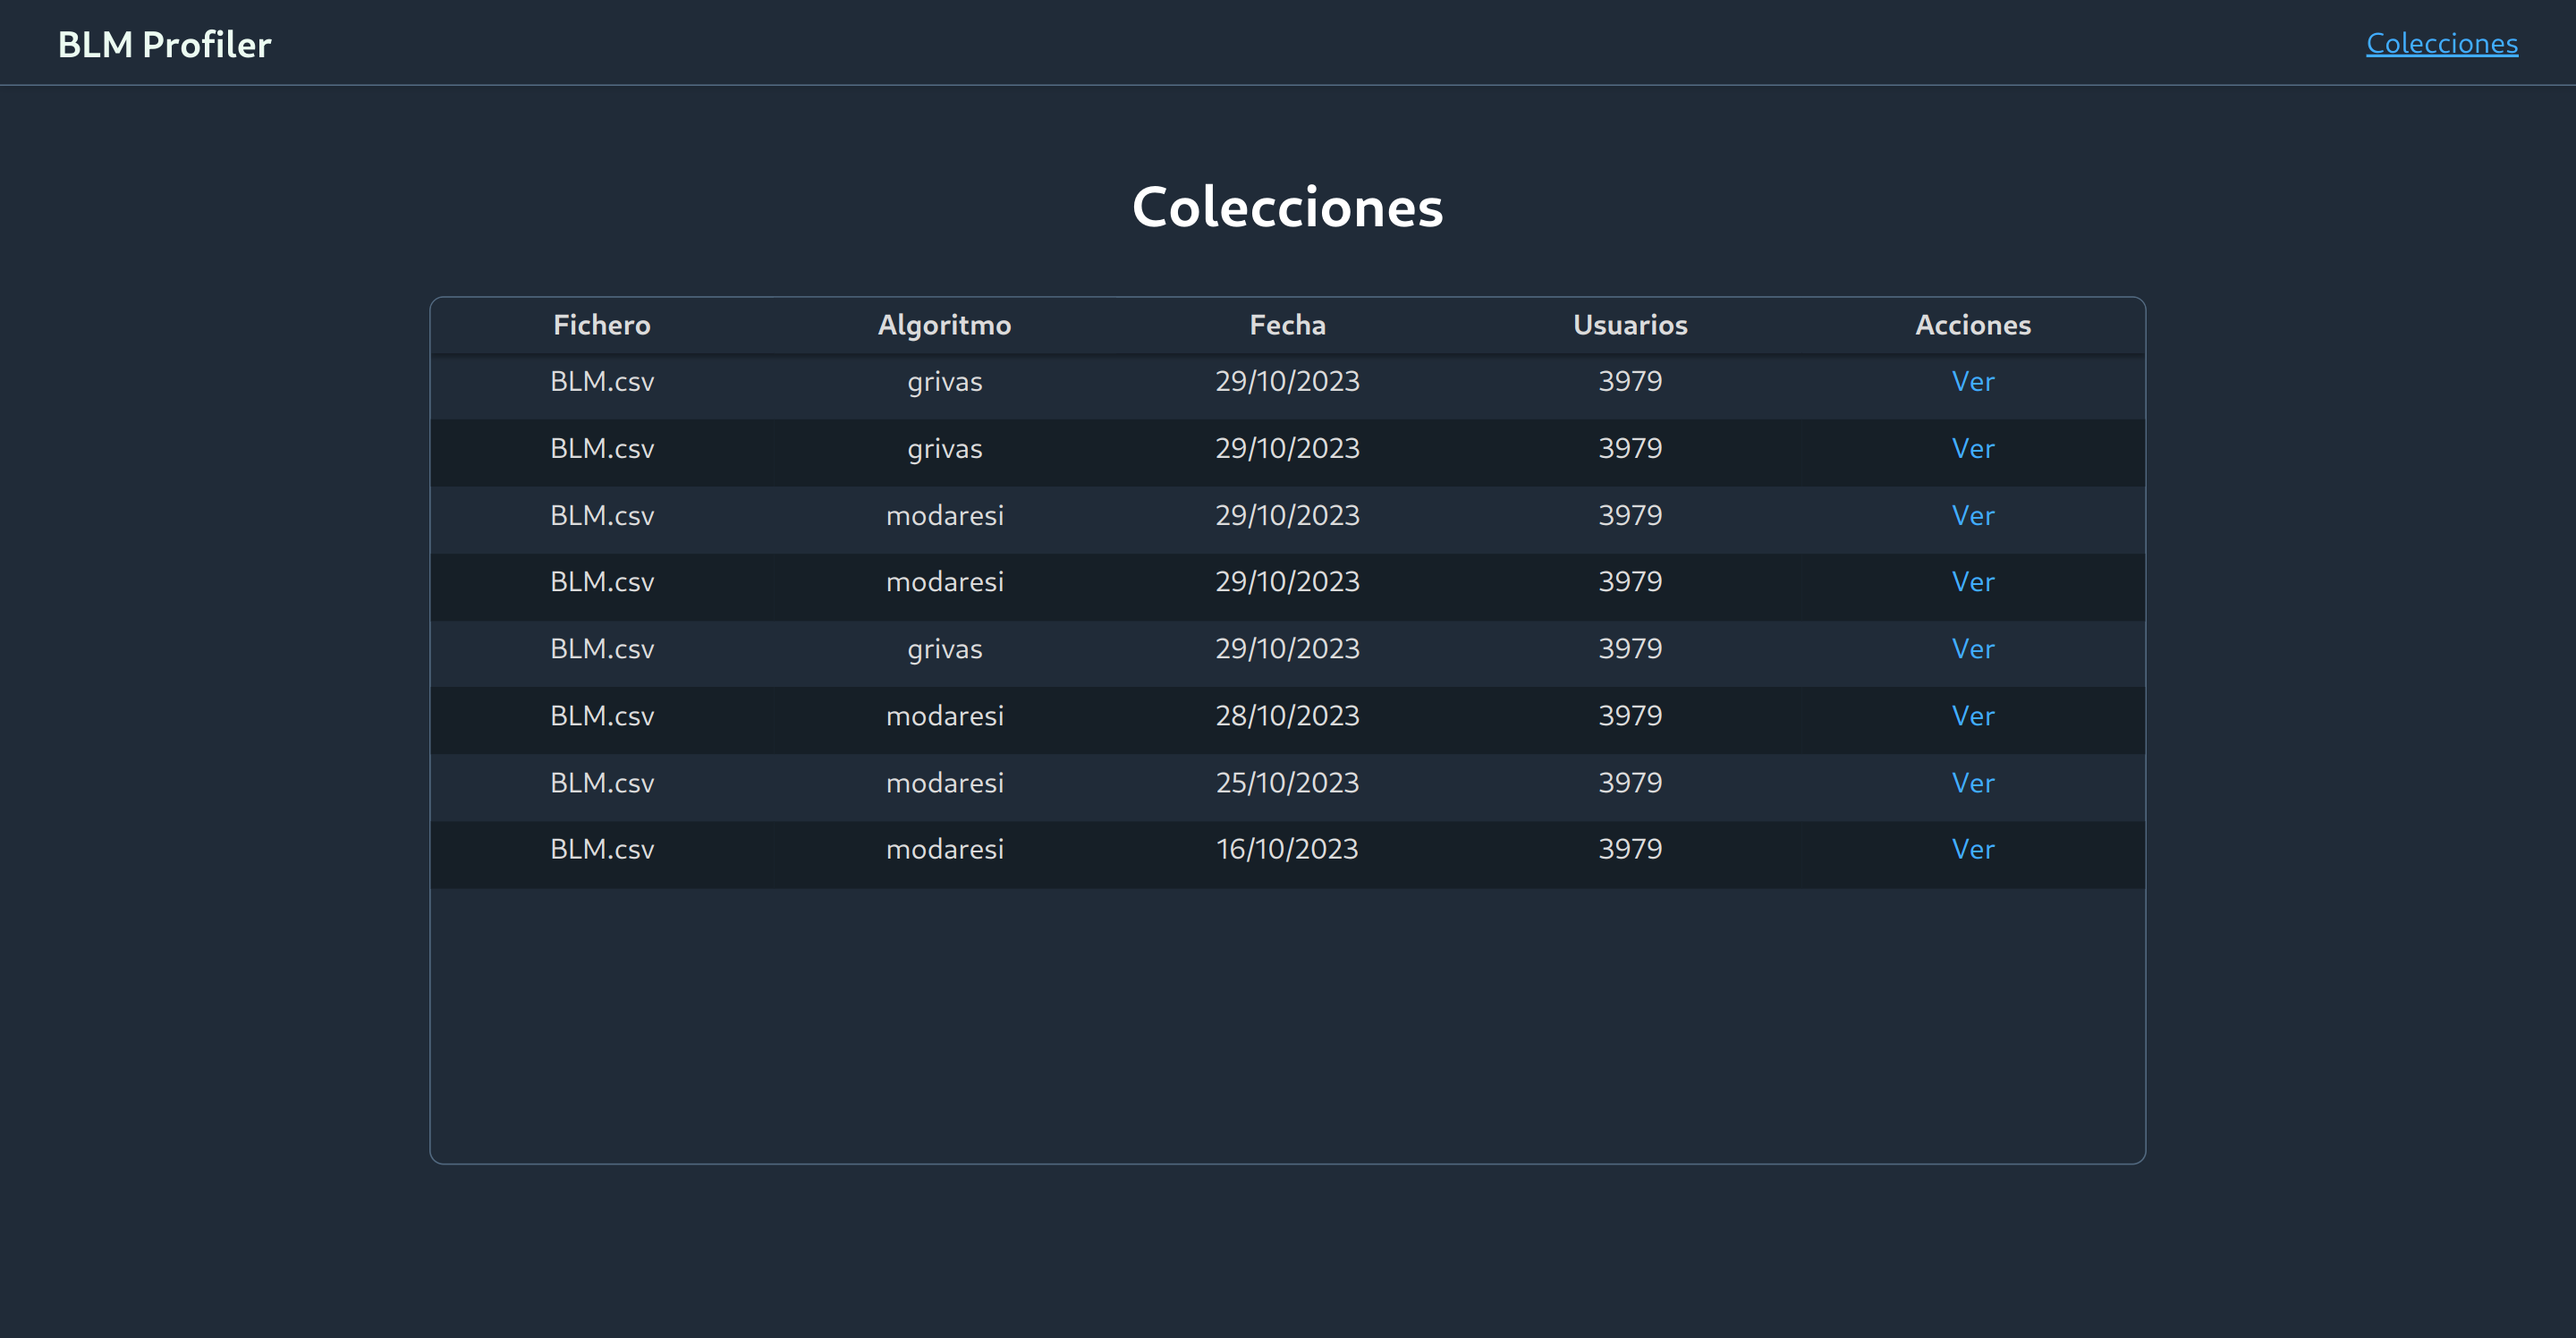
\includegraphics[width=\textwidth]{imaxes/capturas-app/desktop/colecciones.png}
  \caption{\textit{Desktop}} 
  \end{subfigure}
  \begin{subfigure}{0.2115\textwidth}
   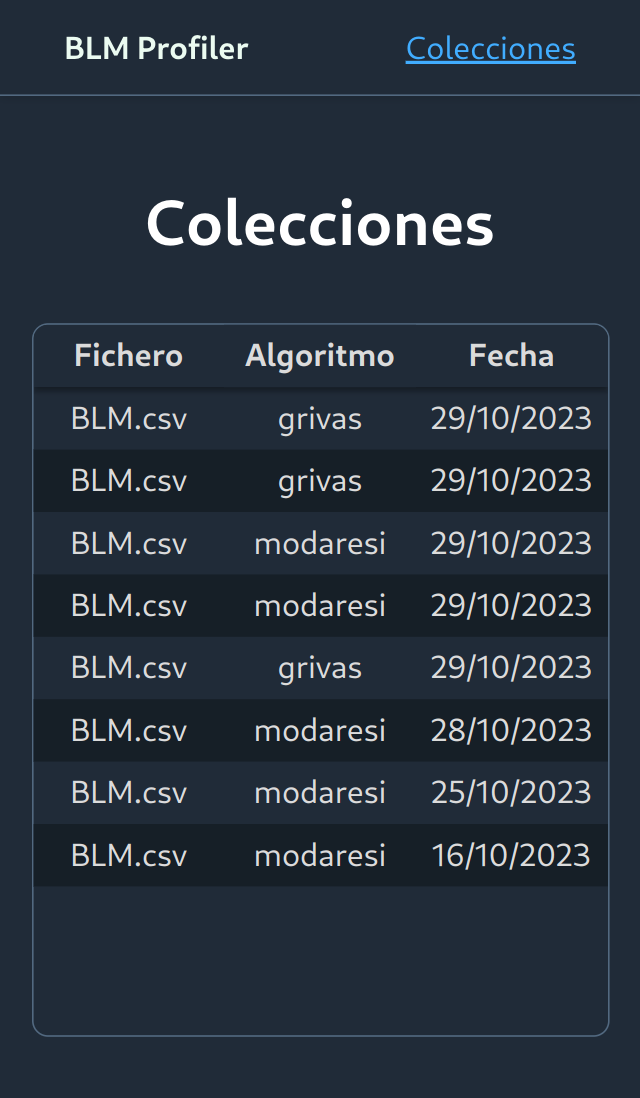
\includegraphics[width=\textwidth]{imaxes/capturas-app/mobile/colecciones.png}
  \caption{\textit{Mobile}} 
  \end{subfigure}
  \caption{Página donde se puede ver el listado de colecciones perfiladas.}
  \label{fig:app/colecciones}
\end{figure}

En esta, tendremos una tabla con las colecciones perfiladas, ordenadas cronológicamente de más a menos recientes. También podremos ver detalles como el nombre del fichero subido, la fecha de subida y el número de usuarios de la colección y algoritmo de perfilado usado en el caso de la versión \textit{desktop}. Asimismo en la columna <<Acciones>> hay un enlace llamado <<Ver>> que nos dirigirá a la página del \textit{dashboard} de esa colección. En la versión \textit{mobile} se puede navegar al \textit{dashboard} tocando sobre la fila de la colección que queramos ver.

\section{Análisis de resultados}

Tras haber explorado el funcionamiento e interfaz de la herramienta de perfilado desarrollada, se procede a una segunda fase en la que se analizan y discuten los resultados obtenidos mediante su uso.

Esta sección se dividirá en un apartado por cada \textit{profiler} utilizado, así como un apartado final a modo de conclusiones generales sobre los resultados de ambos.

Como ya hemos comentado anteriormente en el capítulo \ref{chap:desarrollo}, no hemos incluido finalmente la funcionalidad de perfilado mediante el algoritmo de \citet{loscalis22} explicado en el apartado \ref{subsec:1aprox}, debido al pobre rendimiento del mismo y en mayor medida a la falta de hardware especializado de nuestra máquina local. Por este motivo tampoco hemos analizado los resultados del mismo en esta sección.

\subsection{Algoritmo de \citet{modaresi:2016}}
Vamos a comenzar viendo en detalle los resultados del perfilado mediante el algoritmo de \cite{modaresi:2016}, visto en detalle en \ref{subsec:3aprox}.

En cuestión de edad, se pueden observar las distribuciones de edad obtenidas  por género en la figura \ref{fig:blm/resultados-edad-moda}. Lo primero que llama la atención, es el gran desequilibrio de usuarios en favor del grupo de 25-34 años, el cual supone prácticamente la totalidad de los mismos, un 99.55\% de la colección. Mientras que, los grupos de entre 18-24 y 35-49 solo alcanzan 9 usarios cada uno (menos del 0.3\%) y el grupo de mayores de 50 años se queda vacío. En las distribuciones de usuarios por género se mantiene constante esta tendencia.

\begin{figure}[H]
  \centering
  \begin{subfigure}{0.3\textwidth}
   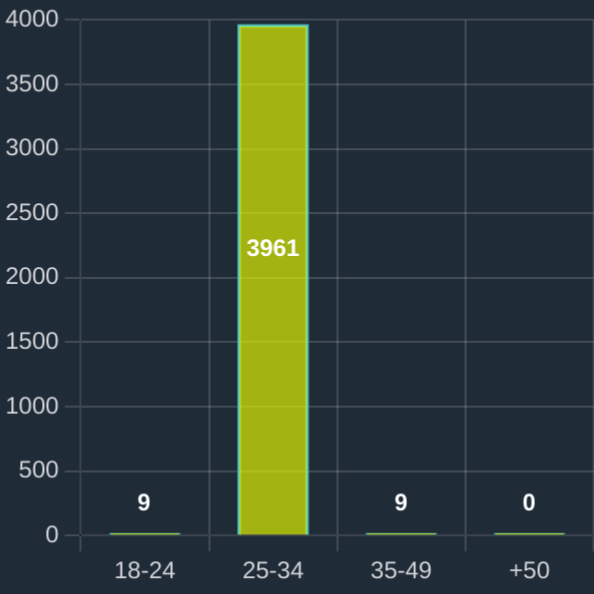
\includegraphics[width=\textwidth]{imaxes/capturas-app/graficos/modaresi/grafico-edad-moda.png}
  \caption{Edad (ambos géneros)}
  \label{subfig:blm/resultados-edad-moda}
  \end{subfigure}
  \begin{subfigure}{0.3\textwidth}
   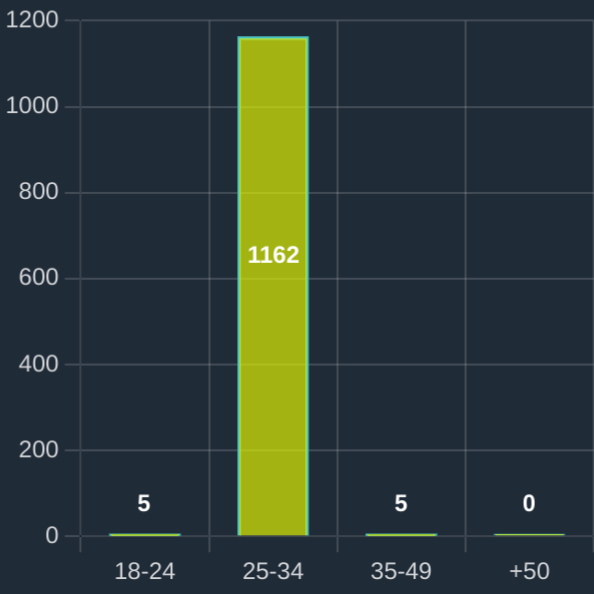
\includegraphics[width=\textwidth]{imaxes/capturas-app/graficos/modaresi/grafico-edad-moda-fem.png}
  \caption{Edad (usuarios femeninos)} 
  \end{subfigure}
  \begin{subfigure}{0.3\textwidth}
   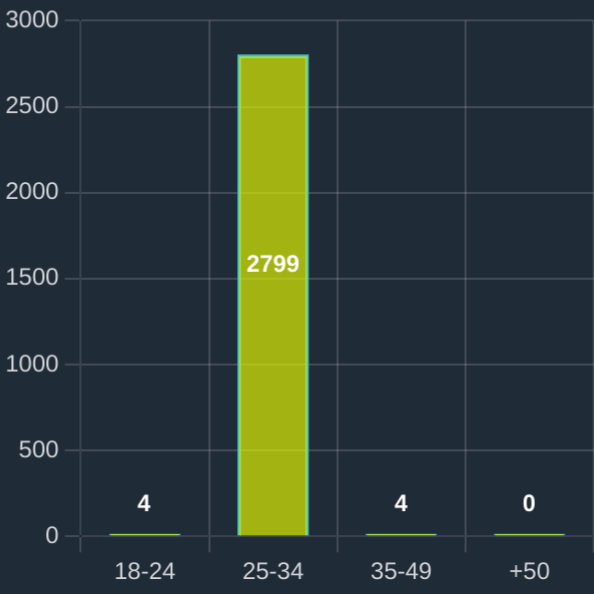
\includegraphics[width=\textwidth]{imaxes/capturas-app/graficos/modaresi/grafico-edad-moda-masc.png}
  \caption{Edad (usuarios masculinos)} 
  \end{subfigure}
  \caption{Distribuciones de edad obtenidas mediante algoritmo de \citet{modaresi:2016}, en corpus \acrshort{blm} en español, según género de usuarios.}
  \label{fig:blm/resultados-edad-moda}
\end{figure}

En cuestión de género, se puede ver en el gráfico en forma de tarta de la figura \ref{fig:blm/resultados-genero-moda} que los usuarios masculinos que publicaban en \acrshort{blm} constituyen casi tres cuartas partes del total de la colección (70.54\%). Sin embargo, si vemos los gráficos por edades podemos darnos cuenta que este desequilibrio solo se da en el rango de edad de entre 25 y 34 años, ya que en el de 18-24 y 35-49 los usuarios femeninos representan más de la mitad en esos grupos demográficos. No obstante, al haber un desequilibro tan grande en cuestión de edad estas mayorías no tienen apenas repercusión en los usuarios totales.

\begin{figure}[H]
  \centering
  \begin{subfigure}{0.3\textwidth}
   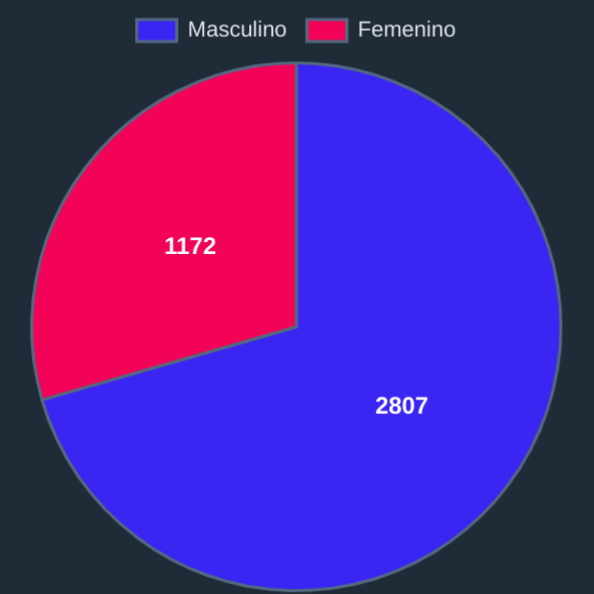
\includegraphics[width=\textwidth]{imaxes/capturas-app/graficos/modaresi/grafico-genero.png}
  \caption{Género (cualquier edad)}
  \label{subfig:blm/resultados-genero-moda}
  \end{subfigure}
  \begin{subfigure}{0.3\textwidth}
   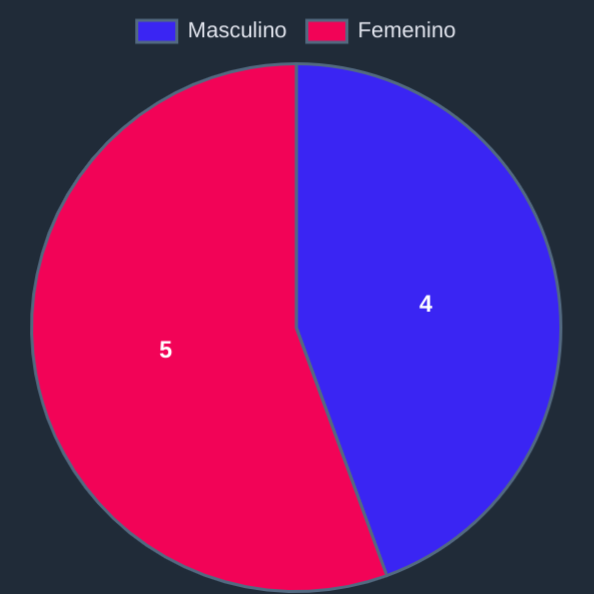
\includegraphics[width=\textwidth]{imaxes/capturas-app/graficos/modaresi/grafico-genero-jj.png}
  \caption{Géner (18-24 años)}
  \end{subfigure}
  \begin{subfigure}{0.3\textwidth}
   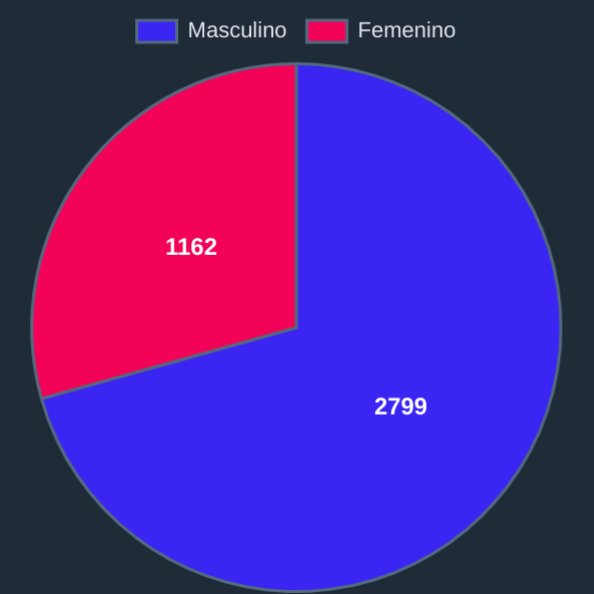
\includegraphics[width=\textwidth]{imaxes/capturas-app/graficos/modaresi/grafico-genero-j.png}
  \caption{Género (25-34 años)}
  \end{subfigure}
  \begin{subfigure}{0.3\textwidth}
   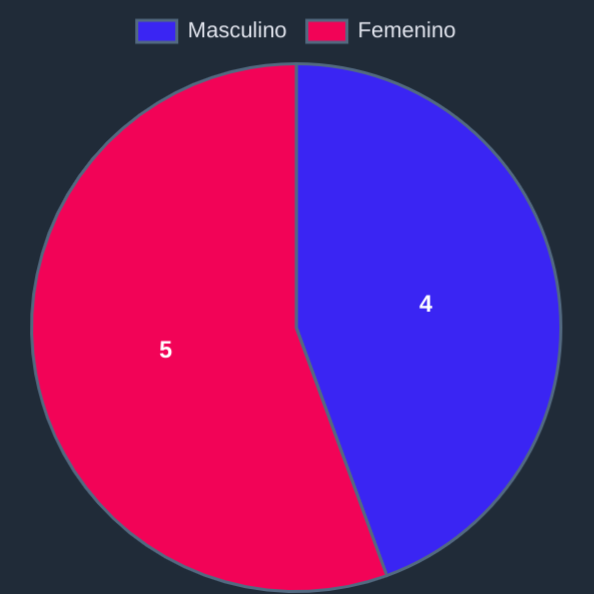
\includegraphics[width=\textwidth]{imaxes/capturas-app/graficos/modaresi/grafico-genero-v.png}
  \caption{Género (35-49 años)}
  \end{subfigure}
  \begin{subfigure}{0.3\textwidth}
   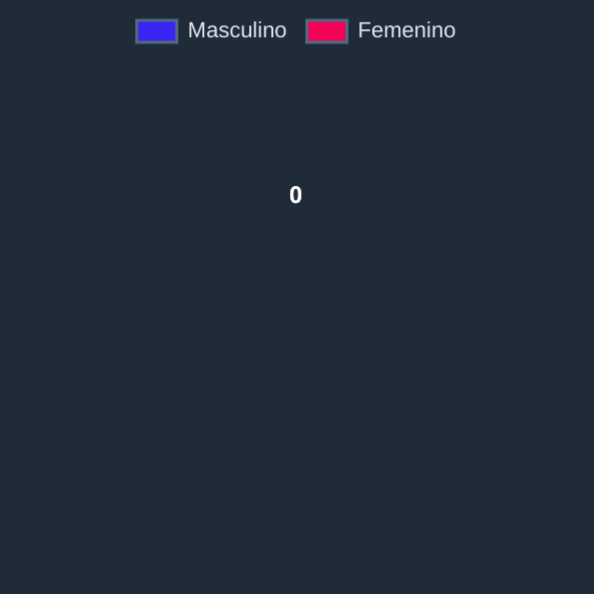
\includegraphics[width=\textwidth]{imaxes/capturas-app/graficos/modaresi/grafico-genero-vv.png}
  \caption{Género (+50 años)}
  \end{subfigure}
  \caption{Distribuciones de género obtenidas mediante algoritmo de modaresi \cite{modaresi:2016}, sobre corpus \acrshort{blm} en español, según rango de edad de usuarios.}
  \label{fig:blm/resultados-genero-moda}
\end{figure}

A modo de resumen, en la tabla \ref{tab:blm/results-moda} se pueden visualizar con detalle la distribución de usuarios en estas dos categorías. Como se podía intuir el grupo demográfico más numeroso es el de usuarios masculinos entre 25-34 años de edad (70.34\%), seguido por las usuarias femeninas de ese mismo grupo cronológico (29.20\%). Otro aspecto resaltable, es la ausencia de usuarios mayores de 50 años.

\begin{table}[H]
    \centering
    \rowcolors{2}{white}{udcgray!25}
    {
    \setlength{\tabcolsep}{0.6\tabcolsep}
    \begin{tabular}{|c|c|c|c|c|c|}
        \hline
        \rowcolor{udcpink!25}
        \diagbox{\textbf{Género}}{\textbf{Edad}} & \textbf{18-24} & \textbf{25-34} & \textbf{35-49} & \textbf{+50} & \textbf{Total} \\ \hline
        \textbf{Femenino} & 5 & 1162 & 5 & 0 & 1172 \\ \hline
        \textbf{Masculino} & 4 & 2799 & 4 & 0 & 2807 \\ \hline
        \textbf{Total} & 9 & 3961 & 9 & 0 & 3979 \\ \hline

    \end{tabular}%
    }
    \caption{Tabla resumen de los usuarios de la colección \acrshort{blm} perfilados mediante algoritmo de \citet{modaresi:2016}.}
    \label{tab:blm/results-moda}
\end{table}

\subsection{Algoritmo de \citet{grivas2015author}}
A continuación se exponen en detalle los resultados obtenidos aplicando el algoritmo de \citet{grivas2015author}, analizado en el apartado \ref{subsec:2aprox} de la memoria.

Comenzando otra vez con la categoría de edad, podemos contemplar de nuevo en la figura \ref{fig:blm/resultados-edad-grivas}, como, aunque ligeramente menor que antes, la gran disparidad de usuarios se mantiene en favor del grupo entre 25-34 años, que aglutina el 97.49\% de la colección. En este caso es el grupo más joven (18-24 años) el siguiente más numeroso con el 2.31\%. Mientras que, de nuevo los grupos de usuarios más mayores, 35-49 y +50 se quedan casi vacíos con 3 y 5 usuarios cada uno. Al examinar estos rangos según el género, se puede apreciar como los usuarios femeninos están bastante más equilibrados, en cuanto a que el grupo de 18-24 representa un mayor porcentaje respecto al total que en el caso masculino (16.67\% por 1.60\%).

\begin{figure}[H]
  \centering
  \begin{subfigure}{0.3\textwidth}
   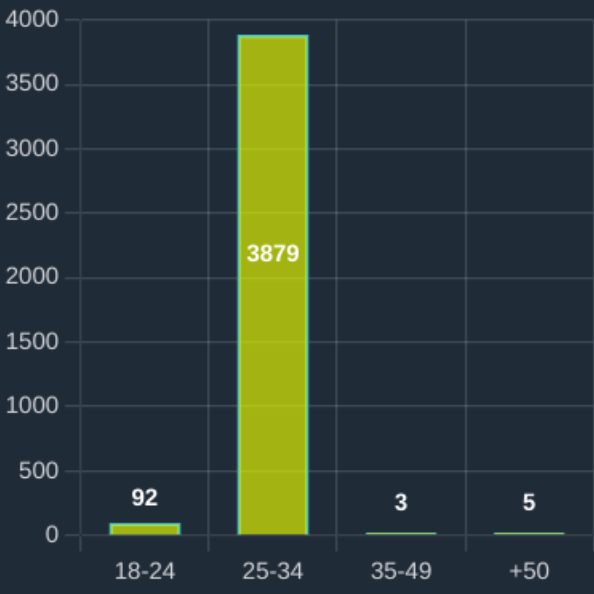
\includegraphics[width=\textwidth]{imaxes/capturas-app/graficos/grivas/grafico-edad-grivas.png}
  \caption{Edad (ambos géneros)} 
  \end{subfigure}
  \begin{subfigure}{0.3\textwidth}
   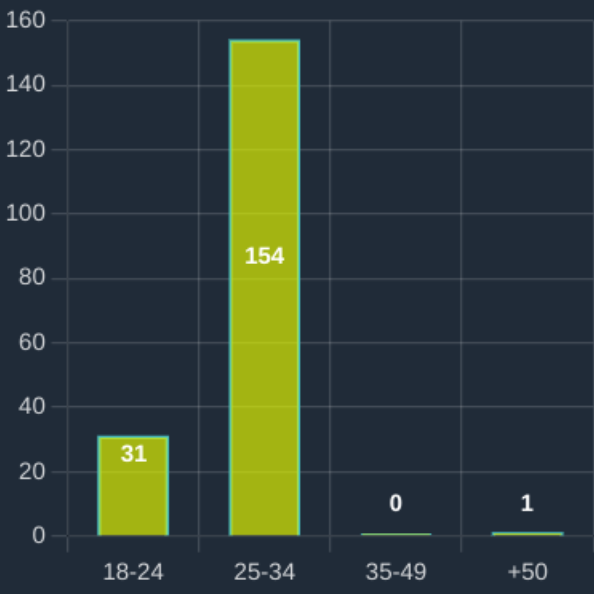
\includegraphics[width=\textwidth]{imaxes/capturas-app/graficos/grivas/grafico-edad-grivas-femenino.png}
  \caption{Edad (usuarios femeninos)} 
  \end{subfigure}
  \begin{subfigure}{0.3\textwidth}
   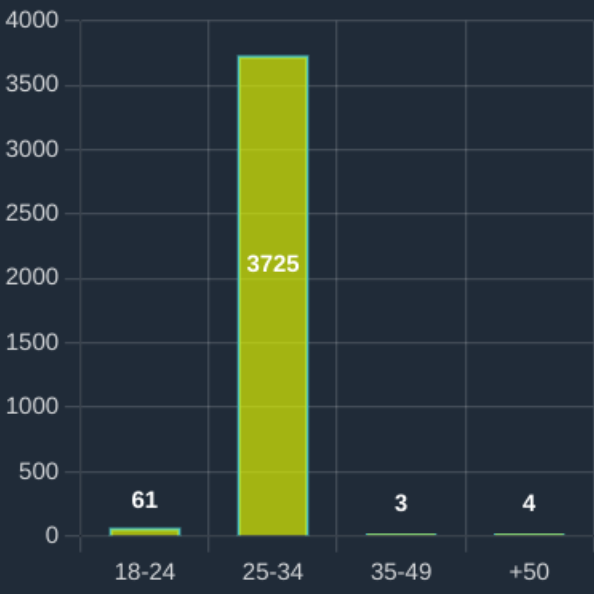
\includegraphics[width=\textwidth]{imaxes/capturas-app/graficos/grivas/grafico-edad-grivas-masculino.png}
  \caption{Edad (usuarios masculinos)} 
  \end{subfigure}
  \caption{Distribuciones de edad obtenidas mediante algoritmo de \citet{grivas2015author}, en corpus \acrshort{blm} en español, según género de usuarios.}
  \label{fig:blm/resultados-edad-grivas}
\end{figure}

Siguiendo con el género, en este caso se puede ver (figura \ref{fig:blm/resultados-genero-grivas}) una mayoría masculina aún más pronunciada que con el algoritmo de modaresi, siendo estos el 95.32\% de la colección. Por grupos de edad se mantiene más o menos igual esta gran mayoría, a excepción del grupo más joven (18-24 años) donde el porcentaje de usuarias crece de el 5 al 33.70\%.
\begin{figure}[H]
  \centering
  \begin{subfigure}{0.3\textwidth}
   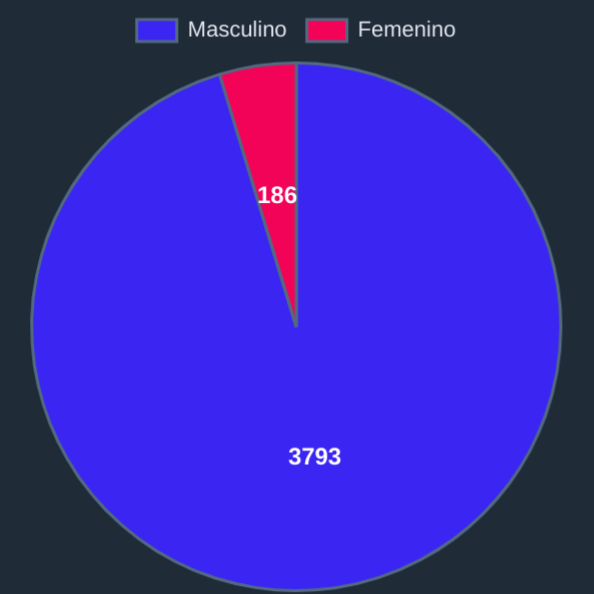
\includegraphics[width=\textwidth]{imaxes/capturas-app/graficos/grivas/grafico-genero.png}
  \caption{Género (cualquier edad)}
  \label{subfig:blm/resultados-genero-grivas}
  \end{subfigure}
  \begin{subfigure}{0.3\textwidth}
   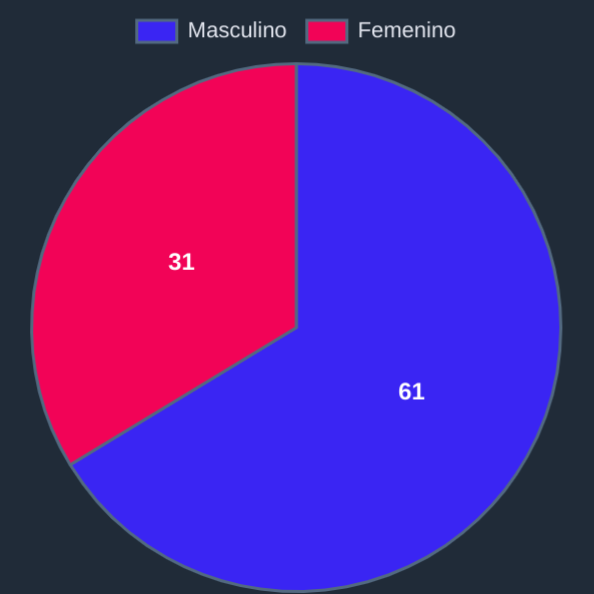
\includegraphics[width=\textwidth]{imaxes/capturas-app/graficos/grivas/grafico-genero-jj.png}
  \caption{Género (18-24 años)}
  \end{subfigure}
  \begin{subfigure}{0.3\textwidth}
   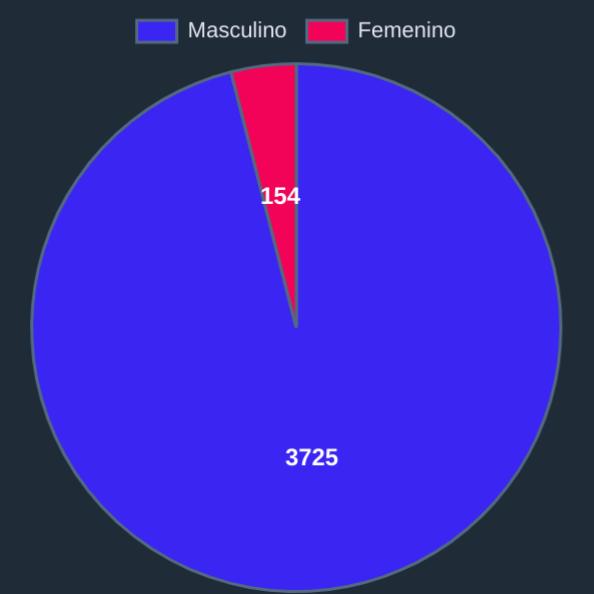
\includegraphics[width=\textwidth]{imaxes/capturas-app/graficos/grivas/grafico-genero-j.png}
  \caption{Género (25-34 años)}
  \end{subfigure}
  \begin{subfigure}{0.3\textwidth}
   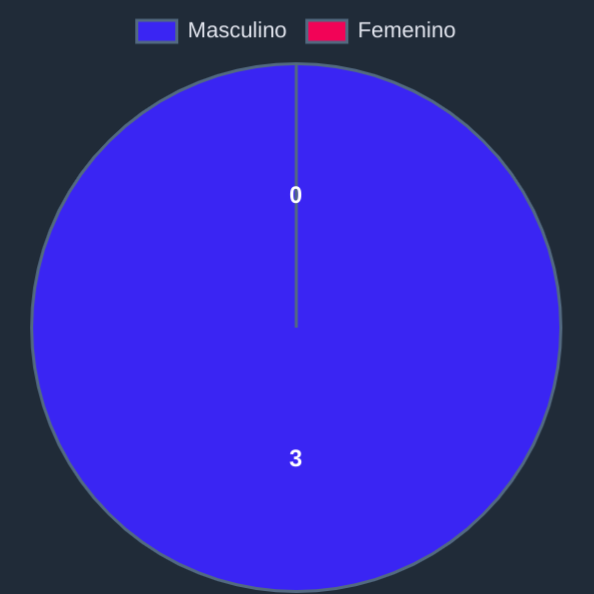
\includegraphics[width=\textwidth]{imaxes/capturas-app/graficos/grivas/grafico-genero-v.png}
  \caption{Género (35-49 años)}
  \end{subfigure}
  \begin{subfigure}{0.3\textwidth}
   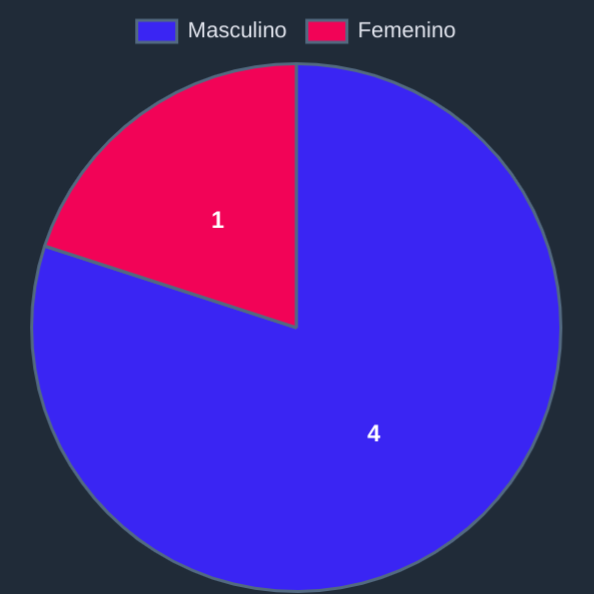
\includegraphics[width=\textwidth]{imaxes/capturas-app/graficos/grivas/grafico-genero-vv.png}
  \caption{Género (+50 años)}
  \end{subfigure}
  \caption{Distribuciones de género obtenidas mediante algoritmo de \citet{grivas2015author}, sobre corpus \acrshort{blm} en español, según rango de edad de usuarios.}
  \label{fig:blm/resultados-genero-grivas}
\end{figure}

Para terminar con este apartado, podemos observar las cifras concretas de usuarios pertenecientes a cada categoría en la tabla \ref{tab:blm/results-grivas}. Como ya adelantábamos, los usuarios masculinos entre 25-34 años predominan en la colección con el 95.38\% seguidos de los femeninos en ese mismo grupo de edad (3.87\%).
\begin{table}[H]
    \centering
    \rowcolors{2}{white}{udcgray!25}
    {
    \setlength{\tabcolsep}{0.6\tabcolsep}
    \begin{tabular}{|c|c|c|c|c|c|}
        \hline
        \rowcolor{udcpink!25}
        \diagbox{\textbf{Género}}{\textbf{Edad}} & \textbf{18-24} & \textbf{25-34} & \textbf{35-49} & \textbf{+50} & \textbf{Total} \\ \hline
        \textbf{Femenino} & 31 & 154 & 0 & 1 & 186 \\ \hline
        \textbf{Masculino} & 61 & 3725 & 3 & 4 & 3793 \\ \hline
        \textbf{Total} & 92 & 3879 & 3 & 5 & 3979 \\ \hline

    \end{tabular}%
    }
    \caption{Tabla resumen según de los usuarios de la colección \acrshort{blm} perfilados mediante algoritmo de \citet{grivas2015author}.}
    \label{tab:blm/results-grivas}
\end{table}

\subsection{Discusión}
En este apartado se hace una discusión acerca de los resultados obtenidos en los dos apartado anteriores. A la vez, se explican las posibles causas de los mismos, así como las implicaciones y conclusiones que se pueden sacar de ellos.

Para empezar, en cuestión de edad ambas aproximaciones apuntan hacia una conclusión parecida: la edad de casi la totalidad de los usuarios que comentaban en \acrshort{blm} está comprendida entre 25-34 años. Siendo el segundo grupo más numeroso el de 18-24 según el algoritmo de \citet{grivas2015author}. Aunque en este último no coinciden ambos algoritmos, es probable que el desequilibrio en cuestión de edad del \textit{dataset} usado para el entrenamiento (\ref{tab:datasets_edad}), haga que estos estén sesgados hacia los grupos de edad más numerosos (25-34 y 35-49). Teniendo en cuenta este hecho, es posible que el desequilibrio en el entrenamiento afecte más a un algoritmo que otro, y por ese motivo el de \citet{modaresi:2016} produce unos resultados tan homogéneos en cuestión de edad. En este sentido, los resultados obtenidos mediante el primer algoritmo \citet{modaresi:2016} parecen estar más influenciados por este equilibrio que los de \citet{grivas2015author}, siendo este último el que alcanza una mayor precisión en las experimentos realizados en cuanto a edad (\ref{tab:aprox2_results}).

Estas conclusiones ganan mayor peso si tenemos en cuenta algunos estudios estadísticos realizados sobre el uso de Reddit, la red social de la que proviene el corpus perfilado. En estos estudios publicados por \citet{reddit2016} se expone como el 59\% de los usuarios de Reddit que participan en temas de actualidad como noticias o discusiones políticas (como es el movimiento \acrshort{blm}), tienen una edad comprendidad entre 18 y 29 años de edad, habiendo otra gran parte de ellos (33\%) entre 30 y 49 años, dejando solo un 7\% restante de mayores de 50.

Por otro lado, los resultados obtenidos en cuanto a género con ambos métodos también nos dejan una conclusión clara: los usuarios varones son  más numerosos que las usuarias mujeres. En este caso, los resultados del algoritmo con mejor rendimiento en los experimentos realizados (\ref{tab:results_aprox3}), como es el de \citet{modaresi:2016}, son los más balanceados que apuntan a un 70\% de usuarios masculinos por el 95\% de usuarios del algoritmo de \citet{grivas2015author}, que quizás muestre un sesgo en favor de este grupo.

Esta proposición va de nuevo en sintonía con los estudios estadísticos sobre Reddit antes mencionados \citep{reddit2016}. En estos se afirma que: los usuarios que se informan y participan en temas de actualidad en la plataforma están constituidos en un 71\% por hombres por un 29\% de mujeres (una distribución de usuarios extremadamente similar a la obtenida con el primer algoritmo). En la figura \ref{fig:blm/estudio-estadistico}, se puede ver una imagen donde se muestran los datos mencionados sobre usuarios de noticias de \textit{Reddit}.

\begin{figure}[H]
  \centering
  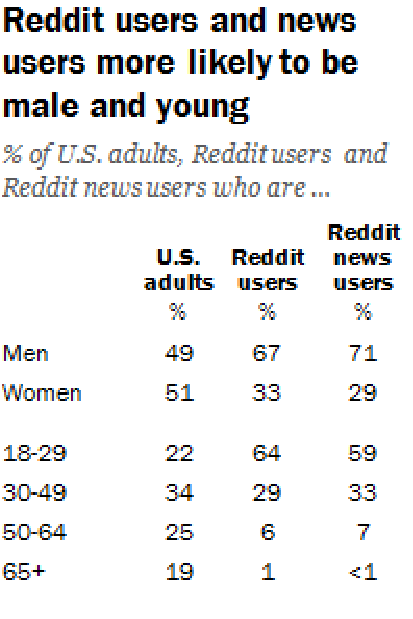
\includegraphics[width=0.3\textwidth]{imaxes/estudio-reddit.pdf}
  \caption{Distribución de usuarios de Reddit según estudio por \citet{reddit2016}.}
  \label{fig:blm/estudio-estadistico}
\end{figure}

En esta línea, podría ser lógico inferir que la distribución de usuarios de Reddit que participan en temas de actualidad, constituya un gran predictivo acerca de la distribución de usuarios en el corpus de referencia.

Por otro lado, un factor importante que limita de manera considerable la fiabilidad de los algoritmos es el hecho de mientras que, la gran mayoría de usuarios tiene pocas publicaciones unos pocos concentran la gran mayoría de \textit{posts} del corpus. En nuestro caso, en el corpus formado por 3979 usuarios, pues 1949 de ellos (el 48.98\% del total) tiene únicamente una publicación en el corpus, 3213 (80\%) tienen menos de 5 publicaciones y 3630 usuarios (más del 90\%) tienen menos de 10 publicaciones en total. Esto se ve ejemplificado por las observaciones de \citet{heritage_BLM} en las que se explica este mismo fenómeno.

La razón por la que este fenómeno limita la fiabilidad de nuestros algoritmos es que: el hecho de no poder contar con una muestra mínima del estilo de redacción de usuario, ocasiona que sea más difícil inferir información sobre el mismo. Así, las predicciones sobre usuarios que cuenten con pocas publicaciones en la colección serán más aleatorias; sucediendo lo contrario al revés: en general, cuantas más publicaciones tenga un usuario, más fiable y menos aleatoria será la predicción sobre el mismo. 

En relación a esto, se puede extraer la siguiente hipótesis: el mayor desequilibrio en edad, se puede ver acentuado por el hecho de que solo se cuente con una publicación para la mitad de los usuarios perfilados. Esto se sustentaría  debido a que los algoritmos no podrán efectuar predicciones lo suficientemente precisas debido a que no cuenta con características relevantes acerca del estos usuarios, haciendo una clasificación más basada en el azar. Esto se puede ver como que los \textit{profilers} no poseen información suficiente para determinar características acerca de un usuario con pocas publicaciones. Esta misma hipótesis es extrapolable al género de los mismos. %Aunque es solemente una conjetura esta podría explicar estos re

Sin embargo, a pesar de esta posible limitación se ha decidido usar la totalidad de usuarios del corpus con motivo de que mostrar los resultados de los usuarios más activos únicamente podría dar lugar a una muestra sesgada y que no fuera representativa del mismo.

\subsection{Comparación con corpus en inglés}

Como se ha comentado en la introducción, una investigación en paralelo ha sido conducida para el la parte de la colección de \acrshort{blm} angloparlante. En este trabajo, \citet{rodriguez_bacelar_automatic_2023} que obtiene unas distribuciones similares a los resultados aquí comentados.

En cuestión de género, los resultados son más acentuados que los aquí comentados: un 94\% de usuarios hombres por solo un 6\% de mujeres. Por otro lado, en edad se obtienen conclusiones contradictorias. Por un lado, mediante un algoritmo se obtiene que una distribución parecida a la nuestra, compuesta por un gran grupo de entre 25-34 años y otro minoritario de 18-24. La otra aproximación, obtiene resultados bastante dispares según el número de publicaciones empleadas por usuario, sin embargo en todas ellas salienta el grupo de 35-49 años como el más común. Este es un resultado peculiar teniendo en cuenta lo comentado anteriormente, sin embargo, el mismo trabajo explica que se puede deber a que el \textit{dataset} usado para entrenamiento (compuesto por celebridades) no es un buen predictor de los usuarios de la colección perfilada.